%%%%%%%%%%%%%%%%%%%%%%%%%%%%%%%%%%%%%%%%%%%%%%%%%%%%%%%%%%%%%%%%%%%%%%
% How to use writeLaTeX: 
%
% You edit the source code here on the left, and the preview on the
% right shows you the result within a few seconds.
%
% Bookmark this page and share the URL with your co-authors. They can
% edit at the same time!
%
% You can upload figures, bibliographies, custom classes and
% styles using the files menu.
%
%%%%%%%%%%%%%%%%%%%%%%%%%%%%%%%%%%%%%%%%%%%%%%%%%%%%%%%%%%%%%%%%%%%%%%

\documentclass[12pt]{article}

\usepackage{sbc-template}
\usepackage[round]{natbib}
\usepackage{amsmath}
\usepackage{color,soul}
\usepackage{graphicx,url}
\usepackage{multicol}
\usepackage{diagbox}
\usepackage[dvipsnames]{xcolor}
\usepackage{verbatim}
\usepackage{makecell}

\newcommand{\R}[1]{~\scriptsize{(#1)}}
\newtheorem{definition}{Definition}
% Keywords command
\providecommand{\keywords}[1]
{
  \small    
  \textbf{\textit{Keywords---}} #1
}


%\usepackage[brazil]{babel}   
\usepackage[utf8]{inputenc}  

     
\sloppy

%\title{SMSM: a Similarity Measure for Trajectory Stops and Moves}
%\author{Andre L. Lehmann\inst{1}, Luis Otavio Alvares\inst{1}, Vania Bogorny\inst{1} }


%\address{Programa de Pós-Graduação em Ciência da Computação \\Departamento de Informatica e Estatistica, Universidade Federal de Santa Catarina\\ Florianopolis, Santa Catarina, Brasil
%  \email{andre.lehmann@posgrad.ufsc.br,alvares@inf.ufsc.br ,vania.bogorny@ufsc.br}
%}

\begin{document} 

%\maketitle

% \begin{abstract}
% For many years trajectory similarity research has focused on raw trajectories, considering only space and time information. With the trajectory semantic enrichment emerged the need for similarity measures that support space, time, and semantics. Although some trajectory similarity measures deal with all these dimensions, they consider only stops, ignoring the moves. We claim that, for some applications, the movement between stops is as important as the stops, and they must be considered in the similarity analysis.
%   In this article we propose SMSM, a novel similarity measure for semantic trajectories that considers both stops and moves.
%   SMSM is evaluated with real trajectory data of CRAWDAD and Geolife. The results show that SMSM overcomes state-of-the-art measures developed for both raw and semantic trajectories.
% \end{abstract}

%\keywords{Trajectory similarity measures, semantic trajectory similarity}

\section{Introduction}
%--vania revisando
Trajectory similarity measuring has received significant attention in the last few years, and several measures have been proposed \hl{to deal either with raw trajectories or semantic trajectories}. A \emph{raw trajectory} is generally represented as a sequence of points $T=<p_1, p_2, ...p_n>$, with $p_i=(x_i,y_i,t_i)$ where $x,y$ is the position of the object in space at time instant $t$.  Examples of similarity measures for raw trajectories are LCSS (Longest Common SubSequence) \citep{vlachos2002discovering}, EDR (Edit Distance on Real sequences) \citep{Chen:2005:RFS:1066157.1066213}, NWED (Normalized Weighted Edit Distance) \citep{dodge2012} and UMS (Uncertain Movement Similarity) \citep{Furtado-UMS-2018}. LCSS \citep{vlachos2002discovering} and EDR \citep{Chen:2005:RFS:1066157.1066213} consider the sequence, but they force a match in all dimensions, not allowing partial similarity between trajectory points.  %\hl{Multi-Dimensional Dynamic Time-Warping} (MD-DTW) \cite{ten2007multi} is another approach that is able to handle multiple dimensions. It extends \hl{Dynamic Time-Warping} (DTW) \cite{berndt1994using} in order to find the distance between two sequences by looking for the best contiguous match of elements according to the sum of the distances in all dimensions. The problem of DTW and MD-DTW is that they consider the real distance between the elements, are sensitive to noise, and were developed for numerical attributes, not dealing with semantic information. 
UMS \citep{Furtado-UMS-2018} is a parameter free method that considers only the spatial dimension, but it outperformed all previous works for raw trajectory similarity.


Existing works for raw trajectory similarity are limited to the spatio-temporal properties of raw trajectories, basically considering trajectories as objects with only space information or space and time.

In 2008, emerged the concept of semantic trajectories \citep{Spaccapietra:2008:CVT:1347466.1347785}, where trajectories are represented as \emph{sequences of stops and moves}. \emph{Stops} are the most important parts of trajectories, representing the places that an object has visited for a minimal amount of time, and the \emph{moves} are the trajectory points between stops. In several works, stops are called points of interest (POIs), episodes, or stay points. Semantic trajectories are more complex than raw trajectories, because they have at least three dimensions: space, time, and semantics. \hl{We consider in this paper that semantics is any type of information associated to mobility data other than spatial location and time.}

\hl{The enrichment of trajectories with semantic information is a well studied topic in the literature, and a number of methods have been developed for this purpose, as the works of} \cite{alvares2007model}, \cite{Palma2008}, \cite{manso}, and \cite{fileto2013baquara}. Aplications as DayTag \cite{fernando2013} can detect stops and moves and the user can add the semantics to his/her trajectories. \hl{Examples of semantic information related to the stops can be, for instance, the name of the stop (e.g. Ibis Hotel) and the category (e.g. Hotel, Museum, Restaurant), while the semantic information related to the move could be, for instance, the name of the streets followed by the moving object and the category of the transportation mode. The explosion of social media data, internet channels, and the facility to enrich trajectories with more context information as linked open data, allows the representation of movement in a more meaningful way. From social media data, for instance, a stop at a hotel can be enriched with the information of the number of stars, the price average, evaluation rate, facilities, parking, wifi, etc.  In this paper we assume that semantic trajectories are represented as sequences of stops and moves, as originally defined in }\cite{Spaccapietra:2008:CVT:1347466.1347785}\hl{, and the way how these trajectories are generated or enriched is out of the scope of this paper.}

\hl{Only a few  similarity measures were proposed for semantic trajectories, as } \cite{Kang:2009:SMT:1529282.1529580}, \cite{Liu:2012:SMM:2442968.2442971}, \cite{Ying:2010:MUS:1867699.1867703}, and \cite{Furtado:TGIS12156}\hl{. The main problems of these measures are that they do not address all three dimensions (space, time and semantics), as the works of }\cite{Kang:2009:SMT:1529282.1529580} and \cite{Liu:2012:SMM:2442968.2442971}\hl{; or, 
they exclusively address the stops, systematically ignoring all information about the moves, as the works of }\cite{Ying:2010:MUS:1867699.1867703} and \cite{Furtado:TGIS12156}\hl{. To the best of our knowledge, none of the existing similarity measures for semantic trajectories have considered both stops and moves. The measure MSM (Multidimensional Similarity Measure) }\citep{Furtado:TGIS12156}\hl{, for instance, considers only the stops, and they are treated as elements that are independent from each other, without considering the order/sequence as they appear in the trajectories. However, MSM ignores the moves between stops. MSM can be used to answer questions like: \emph{how similar are two trajectories $P$ and $Q$ considering their stops?}}
%In the example shown in Figure {\ref{fig:Paris}}, that shows the trajectories of three tourists visiting the same places (stops S1, S2, S3 and S4) in Paris, MSM would give a similarity degree of 100\%, because the objects visited the same places and MSM ignores the moves.

 

\hl{Similarity measures are the basis of several data processing and analysis techniques, such as information retrieval, location prediction, nearest neighbour queries, outlier detection, clustering, etc. A clustering algorithm, for instance, uses a similarity measure for grouping objects with similar trajectories. Outlier detection methods use similarity to find groups of trajectories with normal behavior, and the objects that are dissimilar to the majority, are the outliers. To detect specific trajectory patterns such as flocks }\citep{Laube2005}\hl{, for instance, a raw trajectory similarity measure could be applied to find a minimal number of objects moving together in space and time. Similarity measures that consider both stops and moves can be important in a vast number of applications such as public transportation systems, traffic management, fraud detection, tourism, urban planning, etc. }
%To mention a few examples, similarity measures are the basis for finding objects that follow the same routes, tourists that visit similar places at similar times, to distinguish categories of users such as students from professors at a university, to find similar taxi trajectories, to find users that use the same means of transportation when visiting the same places, etc.


\begin{figure}[h]
\label{fig:Paris}
\centering
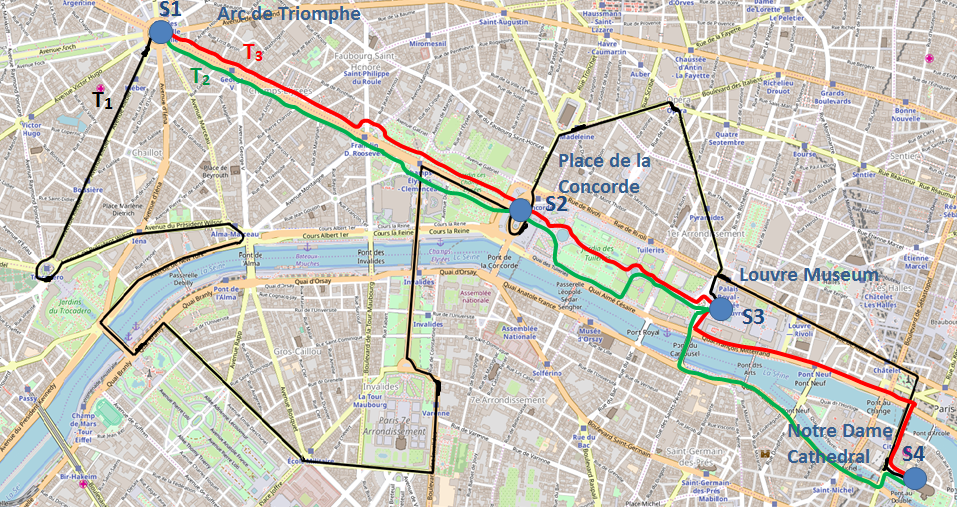
\includegraphics[width=1.0\textwidth]{Images/paris5.png}
\caption{Tourist trajectories in Paris with four stops}
\end{figure}


\hl{To better understand the need for considering both stops and moves in trajectory similarity analysis, let us consider the example in Figure {\ref{fig:Paris}}, for a tourism application, which shows three trajectories of tourists visiting Paris. These tourists visited four places, in this order:  Arc de Triomphe (first stop - S1), Place de la Concorde (second stop - S2), the Louvre Museum (third stop - S3), and the Notre Dame Cathedral (the last stop - S4). The three tourists visited the same places at the same order, but the tourists of trajectories $T2$ (green trajectory) and $T3$ (red trajectory) moved on foot, following the shortest path, while the tourist of trajectory $T1$ used a city tour hop on and hop off bus to appreciate the view. The question we want to answer in this paper is \emph{how similar are trajectories $T1$, $T2$ and $T3$ considering both stops and moves?} From the figure it is clear that trajectories $T2$ and $T3$ are more similar, because they used almost the same paths between stops and moved on foot, while trajectory $T1$ has a completely different move. Now suppose that a tourism manager wants to recommend a trip to a new tourist arriving in Paris, and this new tourist wants to visit the same places visited by the tourists in the figure, but he wants to move on foot and follow the path used by the majority of the tourists.
For this case, we need to retrieve trajectories $T2$ and $T3$. 
%Another example is to calculate the proportion of tourists that visit these four stops moving on foot in order to eventually propose a new hop on hop off tourist bus line.
Another example is the evaluation of the flow of tourists moving on foot between these four stops in order to eventually propose a new and direct hop on hop off tourist bus line.}
%Another example is a tourism manager that wants to send advertisements for pedestrians about a new restaurant at Champs Elysées Avenue between \emph{Arch de Triomphe} and \emph{Place de la Concorde}.}
%From the whole database of trajectories, a query must return the most similar trajectories to the trajectory that this new user wants to perform. It is clear that for this problem, a good recommendation is only possible if we consider the sequence of visited places, the duration of the visits, the real path followed during the move, as well as the move transportation mode. 

\hl{In taxi fraud detection, for instance, a similarity measure will help to answer questions like: given two regions of interest, which is the standard path followed by the majority of the taxis and which are the outliers?
%to find a taxi fraud trajectory between two given stops, a similarity measure must be used to find the standard path that connects the stops, for then identifying the outlier trajectories. 
A real example of an outlier taxi trajectory is shown in Figure {\ref{fig:crawdad_outlier}}, in the San Francisco dataset of the Crawdad project} \citep{epfl-mobility-20090224}. \hl{In this example, given the stops Airport and  Westfield San Francisco Centre (WSFC), a similarity measure must consider both stops and moves to find the black trajectories as the most similar movements between the Airport and WSFC, and the trajectory in purple as the most dissimilar trajectory, which made a completely different and longer trip.}
 
\begin{figure}[h]
\centering
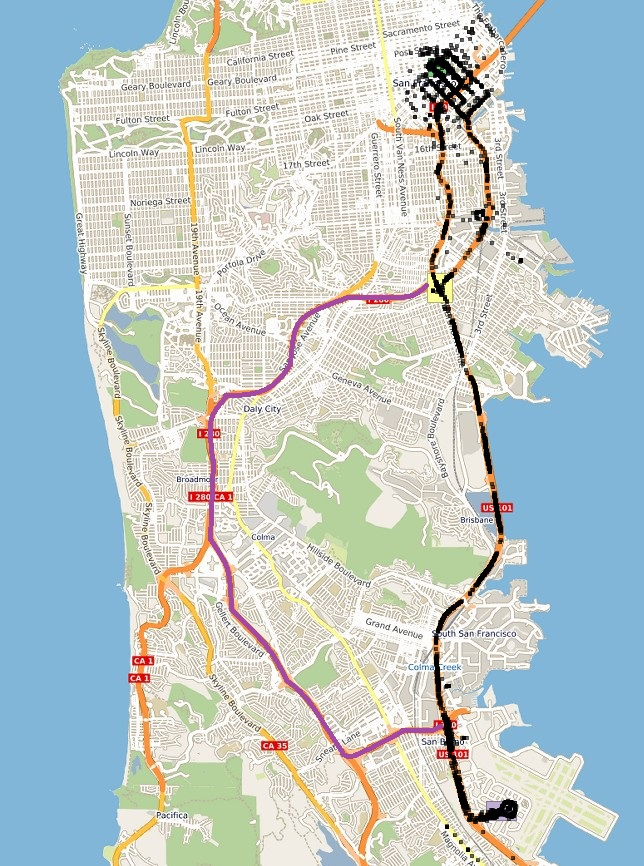
\includegraphics[width=0.5\textwidth]{Images/CRAWDAD-Outlier.jpg}
\caption{\label{fig:crawdad_outlier} An outlier trajectory (in purple) going from Airport to downtown of San Francisco}
\end{figure}


%We claim that for several applications, the moves are as important as the stops, or even more important. Moves carry important information such as the traveled distance from one place to another, the transportation means, the name of the streets followed by the moving object, the average speed, etc. Moves are important for answering semantic queries that involve both stops and moves such as (i) which objects go from a stop A (e.g. city center) to a stop B (e.g. airport) through the same roads? Which is the most popular route from A (e.g. city center) to B (e.g. University x)?}

%Answering this kind of question is important in several applications. In car sharing systems, for instance, the origin and destination of the trip is important, but the path followed between the origin and destination is important as well, in order to find ride intersection. In public transportation systems, both bus stops and streets must be known to propose new bus lines. In traffic management applications, the moves between spatial regions must be used to detect traffic jams.

In all previous examples MSM cannot distinguish the trajectories, because it ignores the moves, and gives a similarity degree of 100\% for the trajectories in both scenarios.
Given the need of spatio-temporal similarity measures that consider both stops and moves, in this paper we propose a new semantic trajectory similarity measure that extends MSM, proposed in \cite{Furtado:TGIS12156}, to support both stops and moves. Our approach considers the sequence of the stops, what is not supported by MSM, allows different semantics for the moves, and uses weights to provide importance degrees for stops, moves, and their attributes. 
In summary, we make the following contributions:
(i) we propose a new similarity measure for multidimensional sequences treating elements with heterogeneous dimensions, which is the case of stops and moves; (ii) the semantic similarity measure considers both \textit{stops} and \textit{moves}, as well as their space, time, and semantic dimensions, allowing the use of different distance functions for each dimension, making the measure robust for several applications; (iii) the measure is flexible enough to consider the order between stops and to support different weights for stops, moves, and dimensions, allowing to give more or less importance to different trajectory parts; (iv) we evaluate the proposed measure with experiments over synthetic and real data, comparing our proposal to a large number of measures developed for semantic or raw trajectories.

The rest of this article is organized as follows: Section \ref{sec:related} presents the related works, Section \ref{sec:proposed_measure} presents the proposed similarity measure with a running example, Section \ref{sec:experiments} presents experiments over real \hl{and synthetic} trajectory data, Section \ref{sec:discussion} presents a discussion about the choice of a measure in face of application problems, and Section \ref{sec:conclusions} concludes the article.

%\hl{Similarity measures play a important role in geospatial information systems, as a tool to analyze the closeness of elements. As an example, we can use a public transportation system. To define a creation of a new bus stop some characteristics should be analyzed: (i) the current usage rate of the bus line; (ii) the growth of population in the region; (iii) the usage rate of alternatives transportation means, as car-pooling systems and taxis; (iv) the size and count of important community buildings, as schools, hospitals, public administrative buildings, etc. So, if a bus line has as characteristic a lower usage rate and near of it occurs a higher usage of other transportation means as car-pooling or taxi, it is expected that the creation of a bus stop will rise the usage rate of buses at the expense of car use. It can reduce traffic jams in the region, it may reduce the air pollution in the city, in addition of being more financially advantageous for passengers. But to define exactly where the bus stops should be created, first of all it is necessary to find out which bus lines cover the region and which are the bus stops shared between them. We use the bus stops as the \emph{stops} and the street names as the \emph{moves} in the stop and move model. After modeling our semantic trajectories, we can find the best place to put a new bus stop by finding a \emph{move} which can be split in two segments, creating a \emph{stop} (the new bus stop) between them. If this new simulated trajectory is more similar to original trajectories, it indicates that the bus line will be slightly changed, having little impact on the mesh of bus lines as a whole.}




\section{Related works} \label{sec:related}
Along the last years, many similarity measures for trajectories were proposed, focusing on raw trajectories, which find the similarity between two trajectories considering spatial and temporal information. \cite{vlachos2002discovering} proposed LCSS, a measure in which two points \textit{match} when their distance is less than a given threshold. The longer the common subsequence of matches between two trajectories, the more similar they are.

\hl{Edit Distance with Real Penalty (ERP) was proposed for time series in }\cite{Chen:2004:MLE:1316689.1316758}\hl{.  It is a marriage of L1-norm and the edit distance. ERP uses real penalty between two non-gap elements, but a constant value for computing the distance for gaps. 
%It computes the distance between two sequences of points by aligning the sequences in a $L_p$-norm space and uses a $L_p$-norm distance function to compute the similarity of sequences. 
As it computes the distance based on the absolute distance, ERP is affected by noisy points in the sequences.} \cite{Chen:2005:RFS:1066157.1066213} proposed EDR, a similarity measure for raw trajectories that calculates the edition difference between the points, as classical edit distance measures. Another measure for raw trajectories is \hl{w-constrained discrete Frechet distance} (wDF) \citep{Ding:2008:ESJ:1440463.1440989}, that considers only the spatial dimension. 

LCSS and EDR have not been proposed for semantic trajectories, but both measures can be easily extended to handle other dimensions (e.g. semantics). However, that extensibility does not allow the measures to represent semantic trajectories as a sequence of heterogeneous elements, that is the case of stops and moves, because both LCSS and EDR demand that all trajectory elements should be homogeneous.

The distance measure Dynamic Time-Warping adaptive (DTWa) proposed in \cite{Shokoohi-Yekta2017} extends the classical \hl{Dynamic Time-Warping} (DTW) \citep{berndt1994using} distance measure to multiple data dimensions. The problem of DTWa is that it deals with numeric dimensions only, and it is a distance function, not a similarity measure.

\hl{UMS was proposed in }\cite{Furtado-UMS-2018}\hl{ as a new parameter-free similarity measure for raw trajectories. UMS was designed exclusively for raw trajectories, considering only the spatial dimension. The major contribution of UMS is that no distance threshold is needed, and the distance between two trajectories is computed with ellipses over every two trajectory points, so trajectories are represented as sequences of ellipses. The similarity is given by the proportion of ellipse intersection. As the ellipses are dynamically defined according to the point distance, UMS solves the problem of trajectories with distinct or varied sampling rates, by computing each ellipse size as big as necessary to cover two consecutive points. UMS outperformed all state-of-the-art works for raw trajectories developed before 2018, so it is currently the best similarity measure for raw trajectories where the spatial dimension is the most important.}

%\hl{Distinctly of the raw points measures, in the work of }\cite{Laube2005}\hl{ a raw trajectory is analyzed through the derived features of the movement, such as speed changing, momentous speed and others. The main purpose of work of Laube is to define a few behavior patterns in raw trajectories and find spatial encounters in respect to these behaviors. Using the REMO concept (RElative MOtion), it approach has as constraint that analyzed trajectories must be synchronized in time. This is not the case in real life trajectories of persons or regular vehicles, since each moving object (person, vehicles, etc) starts its movement independently each other, limiting it uses for some specific contexts, such as birds migration, wildlife monitoring, etc. In a similar way, the work proposed in } \cite{Shirabe2006}\hl{ shows that a strong correlation of motion features can help to find a linear correlation between trajectories in raw trajectory datasets. A drawback of the approach is the inability to consider the spatial and temporal location of each point. In other words, the trajectories are analyzed only by their behavior and not by their discrete points.}

The Common Visit Time Interval (CVTI) is proposed in \cite{Kang:2009:SMT:1529282.1529580} as a measure to integrate the semantic dimension of the stops with the temporal dimension. Although using different data dimensions, the measure is not extensible for other dimensions associated with the point, not allowing heterogeneous data such as stops and moves to be modeled and measured together.

In \cite{Ying:2010:MUS:1867699.1867703} the measure \hl{Maximal Semantic Trajectory Pattern} (MSTP) is proposed, which despite being a measure for semantic trajectories, it is not able to handle multiple data dimensions. Moreover, as MSTP essentially works with the frequency at which stops are visited, it is not able to consider moves between stops.

In the work of \cite{Furtado:TGIS12156}, the MSM measure is proposed to multidimensional similarity measuring, and it is so far, the best similarity measure for semantic trajectories. In MSM all elements must be homogeneous, not allowing the representation of heterogeneous elements as stops and moves. MSM is more robust than LCSS and EDR by allowing partial dimension matching and not forcing a sequence. MSM was developed to work only with stops, and the sequence of elements is not taken into account during the similarity calculation, ignoring the order of the stops. We claim that for some applications as car sharing, new bus route planning, traffic analysis, and recommendation systems, the sequence of stops may play an important role.

%=====================================================================================
%======================================================================================


\section{The Proposed Measure: SMSM} \label{sec:proposed_measure}
In this section we present a novel similarity measure to consider both stops and moves of semantic trajectories, called SMSM (\textit{Stops and Moves Similarity Measure}). The idea behind SMSM is a measure that overcomes the strictness of LCSS and EDR by allowing partial order and dimension matching, and the limitations of MSM by considering both stops and moves. Before we introduce the concepts related to the new measure, we formally define semantic trajectory, considering its sequence of stops and moves, which is an enriched extension of the definition presented in \cite{Spaccapietra:2008:CVT:1347466.1347785}:


\begin{definition}
\label{def:semantic_trajectory}
A semantic trajectory  $ST=\langle s_1, m_1, s_2, m_2, s_3,m_3, ...., s_n, m_n, s_{n+1} \rangle$ is a time ordered sequence of stops and moves, where each stop $s_i$ has a set of attributes $\{d_{s1}, d_{s2}, ...d_{sq}\}$ characterizing it according to q-dimensions, and each move $m_j$  has a set of attributes $\{d_{m1}, d_{m2}, ...d_{mr}\}$  characterizing it according to r-dimensions. 
\end{definition}

In this work we assume that a semantic trajectory starts and ends with a stop, otherwise we transform the first and/or the last point of the trajectory in a stop \hl{as we assume that every trajectory starts and ends at a place}. In the following section we present the new concepts and the definition of the proposed similarity measure SMSM.

\subsection{Basic Concepts and the Proposed Measure}

Stops and moves by definition are different and heterogeneous trajectory elements. A stop may have a spatial position, a start and end time, a category, or a set of attributes related to the category (e.g. Category hotel, stars, rate, price), etc. A move always starts and ends in a stop and may be characterized by different attributes as average speed, traveled distance, sequence of streets, duration, the sequence of raw points, etc. These attributes are defined according to the needs of the application. 

In order to deal with these heterogeneous elements (stops and moves), we introduce the concept of \emph{movement element}. A movement element is a new representation that is not treated by other measures, mainly MSM, which supports only stops. Indeed, MSM does not consider the order of trajectory elements, while in our approach we preserve the sequence of both stops and moves in a movement element.

\begin{definition}
\label{def:movement_element}
A movement element  $e=(stopS, move, stopE)$ is a tuple formed by a start stop $stopS$, the $move$ between $stopS$ and  $stopE$, and the end stop $stopE$, where stopS and stopE are two consecutive stops.
\end{definition}


Hereafter we will consider a semantic trajectory as a sequence of \textit{movement elements}, as follows: 
$ST=\langle e_1=(s_1,m_1,s_2), e_2=(s_2,m_2,s_3), ..., e_n=(s_n,m_n,s_{n+1}) \rangle$.

Notice that we define a movement element as a trajectory part, and this structure will be used for the proposed similarity measure, where one trajectory will be compared with another one based on their movement elements.



We analyze the similarity of a movement element $a\in A$ with another movement element $b\in B$, where A and B are semantic trajectories, in two parts: their stops and their moves. The basis for measuring the similarity of these two parts is the \emph{match} function, given in Equation \ref{func:match1}. The function returns 1 if the distance between an attribute (also called dimension) of two movement elements is less than a given threshold \emph{maxDist}, and zero otherwise. This function is used for measuring the distance of all dimensions of both: the stops and the moves.

\begin{equation}
%\scriptsize
\label{func:match1}
  match_i(a, b) = 
  \begin{cases} 
      1 & dist_i(a, b) \leq maxDist_i \\
      0 & otherwise
  \end{cases}
\end{equation}

To compute a total score for two movement elements $a$ and $b$ we define the function \emph{score(a,b)} in Equation \ref{func:score1}, where, $w_{stop}$ and $w_{move}$ are the weights of the stops and the moves, respectively, and their sum should be one. The importance of either stops or moves can vary from one application to another, so we can use the weights to give the respective importance. 


\begin{equation}
%\scriptsize
\label{func:score1}
score(a, b) = scoreStop(a, b) * w_{stop} + scoreMove(a, b) * w_{move}  
\end{equation}


In our measure we consider a score for the stops (scoreStop) and a score for the move (scoreMove). The functions \emph{scoreStop(a,b)} and \emph{scoreMove(a,b)} are defined in Equations \ref{func:scoreStop1} and \ref{func:scoreMove2}, respectively. In both equations, $r$ and $q$ are the number of dimensions (attributes) of stops and moves, respectively. The score of the stops, computed according to Equation \ref{func:scoreStop1}, is given by the average of all dimension matches of the start and end stops of two movement elements $a$ and $b$. 


\begin{equation}
%\scriptsize
\label{func:scoreStop1}
%\begin{split}
  scoreStop(a, b) = \sum\limits_{i=1}^r (match_i(a_{stopS}, b_{stopS}) + match_i(a_{stopE}, b_{stopE}))\div 2* w_{i}
%\end{split}
\end{equation}


\begin{equation}
%\scriptsize
\label{func:scoreMove2}
\begin{split}
scoreMove(a, b)  & = 
  \begin{cases} 
      \sum\limits_{i=1}^q match_i(a_{move}, b_{move}) * w_{i} & if matchStops(a, b)\\
      0 & otherwise
  \end{cases}
\end{split}
\end{equation}


%The sum of the weights in Equations \ref{func:scoreStop1} and \ref{func:scoreMove2} should be one.
Note in Equation \ref{func:scoreMove2} that the \emph{scoreMove} depends on the function \textit{matchStops(a, b)}. \hl{The intuition is that two moves should be evaluated only if their starting positions (starting stops) are spatially close and the ending positions (ending stops) are close as well.}
The function \emph{matchStops(a,b)} is true when the \hl{spatial distance} between $a_{stopS}$ and $b_{stopS}$  as well as between $a_{stopE}$ and $b_{stopE}$ is less than or equal to $maxDist$.
    
    %\textcolor{red}{In real scenarios, this means that if we want to analyze movement elements, for instance, from France to Italy, we do not need to compare these trajectories with others moving from France to Spain, since the ending stop is different}.

\hl{Figure {\ref{fig:move}} shows an example of four movement elements representing part of four trajectories. The movement elements are $e_1=<A, P_1, B>$, $e_2=<A, P_2, B>$, $e_3=<A, P_3, B>$ and $e_4=<A, P_4, C>$, where $A$, $B$, and $C$ are the stops, and $P_i$ are the moves. Considering $e_1$ and $e_4$, the function $match(P_1,P_4)$ will be executed only if the function $matchStops(B,C)$ is true, i.e., $dist(B,C) \leq  maxDist$. If $dist(B,C) > maxDist$, the value of $scoreMove(e_1,e_4)$ is zero.
%So the \emph{moves} of the movement elements $<A, P_1, B>$, $<A, P_2, B>$, $<A, P_3, B>$ will be analyzed because they have the same start and end stop.}
}

 %and three trajectories move to $B$ following three different paths.  In the example in Figure \ref{fig:move}, if we are interested in trajectories moving from A to B, our measure will only analyze the moves $P1$, $P2$, and $P3$ of trajectories going from A to B, and these three moves will not be compared with $P4$. 

%\hl{Differences among the three movement elements rely exclusively on the differences of the move. On the other hand, the difference of these movement elements to movement element $<A, P_4, C>$ is more evident, since if it end stop is distinct, the move is distinct too. Based on this, SMSM do not compare the move of $<A, P_4, C>$ with the others movement element.}

\hl{The function \emph{scoreMove()} guarantees a partial order in the similarity analysis. %, what has not been considered by MSM, which is the closest measure to our approach, but that considers only stops and without any order. Considering that the four movement elements in Figure {\ref{fig:move}} belong to four different trajectories, MSM would give the same similarity for the parts of the trajectories going from $A$ to $B$, because it does not look the moves, and 50\% similarity with the trajectory going from $A$ to $C$ because they share 50\% of the stops.
Suppose the example in  Figure {\ref{fig:move}} is a real scenario, where $A$, $B$, and $C$ represent  places as France, Italy, and Spain, respectively. We believe that the three trajectories going from France ($A$) to Italy ($B$) must have their move analyzed because they visit the same sequence of places, while the trajectory that goes from France ($A$) to Spain ($C$) does not share the same destination, so the move of this trajectory is not compared with the others, and the function $scoreMove()$ has values zero.}



\begin{figure}[h]
\centering
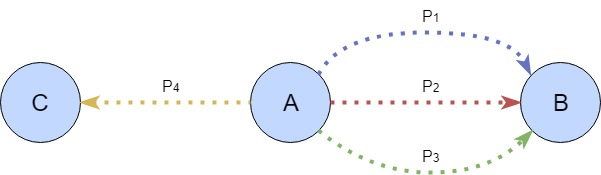
\includegraphics[width=0.75\textwidth]{Images/Toy_trajectories.jpg}
\caption{\label{fig:move} Movement elements: stop $A$ to stop $B$ with the moves $P_1$, $P_2$, and $P_3$; and Movement element: $A$ to $C$ with the move $P_4$}
\end{figure}

Having defined the score for stops and moves for comparing movement elements, Equation \ref{func:parity} defines the parity of two semantic trajectories $A$ and $B$. The parity of $A$ with $B$ is the sum of the highest score of all the elements $a \in A$ when compared with all the elements of $B$.
\begin{equation}
\label{func:parity}
parity(A, B) = \sum\limits_{a\in A} \textbf{max}\{\textit{score}(a, b) : b \in B\}
\end{equation}

Finally, we can define the global similarity of two trajectories $A$ and $B$ with $SMSM$. Equation \ref{func:SMSM1} defines the stops and moves similarity measure $SMSM(A,B)$ by the average parity of $A$ with $B$ and of $B$ with $A$. \hl{The average parity is given by the sum of both parities over the sum of the number of elements in $A$ ($|A|$) and the number of elements in $B$ ($|B|$).}

\begin{equation}
\label{func:SMSM1}
%\scriptsize
\begin{split}
  SMSM(A, B) = 
  \begin{cases} 
      0 & if  |A| = 0 \vee |B| = 0 \\
      \frac{parity(A, B) + parity(B, A)}{|A| + |B|} & otherwise
  \end{cases}
\end{split}
\end{equation}



\subsection{Evaluation over a running example}

In this section we present a running example, comparing SMSM and MSM, since MSM is the closest approach.
Let us consider the two trajectories shown in Figure \ref{fig:bus}. Trajectory $Q$ represents the daily routine of a professor, that starts his day at the gym in the morning, while trajectory $P$ is the daily routine of a student, that starts his day at a coffee shop. Both trajectories visit the same places, sharing some streets, but in totally different order. The trajectories are annotated with the stop category, start and end time of the stop, an hypothetical geographic position ($x, y$) of the stop and the main street followed during the moves. So considering the \hl{notation \textit{stop name ((x, y), [start timestamp - end timestamp])}}, the student has the following movement behavior: stays at \textit{Home} (\textit{(96,215)}, [\textit{8pm-8am}]), \hl{then} he goes via Edu Vieira street to have breakfast at the \textit{Coffee shop} (\textit{(182,201)}, [\textit{8:50am-10am}]), and from there goes via Delfino Conti street to the \textit{University} (\textit{(59,127)}, [\textit{10:25am-6:10pm}]), finishing the day moving via Henrique Fontes street to the \textit{Gym} (\textit{(268,63)}, [\textit{7:30pm-9pm}]). The professor (trajectory $Q$) goes from \textit{Home} (\textit{(13,81)}, [\textit{7pm-7am}]) via Beira-mar avenue for jogging at the \textit{Gym} (\textit{(268,63)}, [\textit{7:30am-8:30am}]). After he goes to the \textit{Coffee shop} (\textit{(182,201)}, [\textit{8:45am-9:55am}]) via Edu Vieira street, and via Delfino Conti reaches the \textit{University} (\textit{(59,127)}, [\textit{10:15am-7:45pm}]) to teach his classes until the end of the day. We have two trajectories $P$ and $Q$ with their stops and moves annotated with the category of the place, the spatial position of the visited place, the time of the visit, and the name of the street to represent the move.
\begin{figure}[h!]
\centering
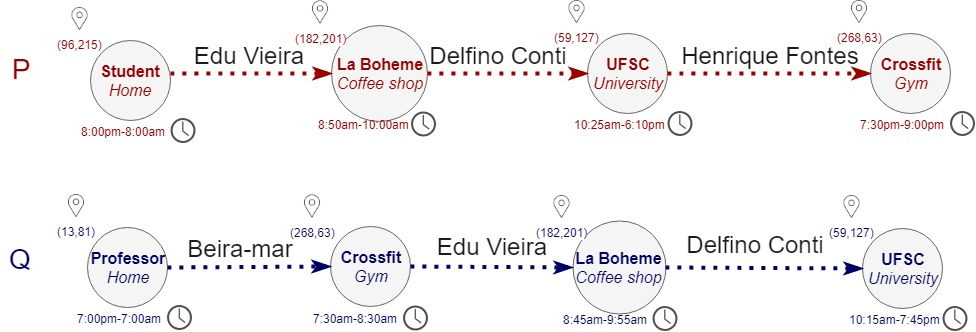
\includegraphics[width=1\textwidth]{Images/running_example.jpg}
\caption{\label{fig:bus} Semantic Trajectories $P$ (Student) and $Q$ (Professor) with stops and moves}
\end{figure}


In order to calculate the SMSM similarity value, we first need to construct all movement elements for each trajectory. Table \ref{tab:SMSM_tuples} lists these elements, where each element contains the start stop, the name of the street followed during the move, and the next stop. 
%Notice in this table that the only movement element where the moves will be analyzed is $<Coffee$ $shop, Delfino$ $Conti, University>$ from trajectory $P$ and $<Coffee$ $shop, Delfino$ $Conti, University>$ from trajectory $Q$, because both start and end stops match.

\begin{table}[h!]
\scriptsize
  \centering
  \begin{tabular}{|c|c|}
  	\hline
		\textcolor{Red}{\textbf{Student (P)}} & \textcolor{Blue}{\textbf{Professor (Q)}}\\
  	\hline
      $<$Home, Edu Vieira, Coffee shop$>$&$<$Home, Beira-mar, Gym$>$\\
      $<$Coffee shop, Delfino Conti, University$>$&$<$Gym, Edu Vieira, Coffee shop$>$\\
      $<$University, Henrique Fontes, Gym$>$&$<$Coffee shop, Delfino Conti, University$>$\\
  	\hline
  \end{tabular}
  \label{tab:wrong}
  \caption{Movement elements}
  \label{tab:SMSM_tuples}
\end{table}

To measure the distance between two movement elements, in this example we use the following distance functions for each stop dimension:
\begin{itemize}
  \item Space: the Euclidean distance between the centroids of the stops;
      \item  Time:  \hl{let $[t1, t2]$ be the time interval of a stop. The time distance of two stops is given by:}
\begin{equation} \label{func:time_interval}
	dist_t(a, b) = 1 - \dfrac{duration([a.t1, a.t2] \cap [b.t1, b.t2])}{duration([min(a.t1, b.t1), max(a.t2, b.t2)])}
\end{equation}
\hl{We use this formula in order to have a proportion of the time intersection and not an absolute value.}
  \item Semantics: the distance is equal to 0 in case of exact match and equal to 1 otherwise.
\end{itemize}

For the sake of simplicity, for the move, in this example we consider only the semantic information, i.e., the name of the followed street, where the distance is equal to 0 in case of exact match of street name and equal to 1 otherwise.
We consider that stops and moves have the same weight and also the dimensions space, time and semantics of the stops.

In this running example we use as thresholds \textit{maxDist\textsubscript{space}} = 100  and \textit{maxDist\textsubscript{time}} = 0.5, i.e. two stops are said as matched in time when both share half of their period in that stop.
With distance functions and threshold values defined and elements constructed, we use Equation \ref{func:score1} to measure the similarity values between all element dimensions, computing first the match in both start and end stops and if the stops match we compute the match for the move. 

To better understand how to measure the movement element similarity let us consider  the following two movement elements: 
\begin{itemize}

\item $element_{P}=\ <Home_{[8pm-8am]}, Edu Vieira,$ $Coffee\ shop_{[8:50am-10am]}>$ ;
\item $element_{Q}=\ <Home_{[7pm-7am]}, Beira-mar, Gym_{[7:30am-8:30am]}>$. 
\end{itemize}
First, we apply the function $match()$ (Equation \ref{func:match1}) for the stops. In this case, the start stops have some degree of similarity: their semantics is the same and the time distance of $Home_{P}$ and $Home_{Q}$ is $\approx 0.15$, lower than our defined threshold of $0.5$. However, the spatial distance is $dist_{eucl}(Home_{P}, Home_{Q}) \approx 158 $, higher than the defined threshold (100), so not matching in space, only in time and semantics, leading to a similarity score of $2/3$ between start stops $Home_{[8pm-8am]}$ and $Home_{[7pm-7am]}$. The end stops (Gym and Coffee Shop) are dissimilar in space (with a distance of $\approx 163$), in time (no overlap), and in semantics, then the similarity score between both end stops is $0.0$.

 Equation \ref{func:scoreStop1} computes the stops similarity as the average similarity of start stops  and end stops as: $scoreStops(element_{P}, element_{Q}) = (2/3 + 0) / 2 \approx 0.33$.
 As the function $matchStops()$ is false in this example since $dist_{eucl}(Coffee$ $shop_{P}, Gym_{Q}) > 100$, when applying Equation \ref{func:scoreMove2}, the function %https://www.overleaf.com/project/5b9ab8c15115371a958f974f 
$scoreMove()=0$. Then, Equation \ref{func:score1} computes the movement element similarity as the sum of stops similarity weighted by $w_{stops}$ and the move similarity weighted by $w_{move}$. In this example, $score(element_{P}, element_{Q}) = (0.33 * 0.50) + (0.00 * 0.50) \approx 0.17$. Table \ref{tab:SMSM_scores} summarizes SMSM similarity scores between all movement elements.

\begin{table}[h]
\scriptsize
  \centering
 \resizebox{\linewidth}{!}{%
  \begin{tabular}{|l|c|c|c|}
  	\hline
		\backslashbox[48mm]{Q}{P}& 
        \makecell{$<$\textcolor{RawSienna}{\textbf{Home}}, Edu V., \textcolor{OliveGreen}{\textbf{Coffee}}$>$ \\ \textcolor{RawSienna}{$[$8pm-8am$]$~~\textcolor{OliveGreen}{$[$8:50am-10am$]$}} \\ \textcolor{RawSienna}{(96,215)}~~~~~~~~~~~\textcolor{OliveGreen}{(182,201)}} & 
        \makecell{$<$\textcolor{OliveGreen}{\textbf{Coffee}}, Delfino C., \textcolor{Mahogany}{\textbf{University}}$>$ \\ \textcolor{OliveGreen}{$[$8:50am-10am$]$}~~\textcolor{Mahogany}{$[$10:25am-6:10pm$]$} \\ \textcolor{OliveGreen}{(182,201)}~~~~~~~~~~~~~~~~~~~\textcolor{Mahogany}{(59,127)}} & 
        \makecell{$<$\textcolor{Mahogany}{\textbf{University}}, Henrique F., \textcolor{Fuchsia}{\textbf{Gym}}$>$ \\ \textcolor{Mahogany}{$[$10:25am-6:10pm$]$}~~\textcolor{Fuchsia}{$[$7:30pm-9pm$]$} \\ \textcolor{Mahogany}{(59,127)}~~~~~~~~~~~~~~~~~~~~\textcolor{Fuchsia}{(268,63)}}\\
  	\hline
      \makecell{$<$\textcolor{RawSienna}{\textbf{Home}}, Beira-mar, \textcolor{Fuchsia}{\textbf{Gym}}$>$\\ \textcolor{RawSienna}{$[$7pm-7am$]$}~~\textcolor{Fuchsia}{$[$7:30am-8:30am$]$} \\ \textcolor{RawSienna}{(13,81)}~~~~~~~~~~~~~~~\textcolor{Fuchsia}{(268,63)}}
      				&0.17&0&0.25\\
      \makecell{$<$\textcolor{Fuchsia}{\textbf{Gym}}, Edu V., \textcolor{OliveGreen}{\textbf{Coffee}}$>$\\ \textcolor{Fuchsia}{$[$7:30am-8:30am$]$}~~\textcolor{OliveGreen}{$[$8:45am-9:55pm$]$} \\ \textcolor{Fuchsia}{(268,63)}~~~~~~~~~~~~\textcolor{OliveGreen}{(182,201)}}
      				&0.25&0&0\\
      \makecell{$<$\textcolor{OliveGreen}{\textbf{Coffee}}, Delfino C., \textcolor{Mahogany}{\textbf{University}}$>$\\ \textcolor{OliveGreen}{$[$8:45am-9:55am$]$}~~\textcolor{Mahogany}{$[$10:15am-7:45pm$]$} \\ \textcolor{OliveGreen}{(182,201)}~~~~~~~~~~~~~~~~~~\textcolor{Mahogany}{(59,127)}}
      				&0.08&1&0\\
  	\hline
  \end{tabular}
  }
  \caption{Similarity scores for SMSM}
  \label{tab:SMSM_scores}
\end{table}

After  computing the similarity scores of both trajectories, with Equation \ref{func:parity} we compute the parity of trajectories, summing the highest scores of all movement elements of one trajectory when compared with all elements of the other trajectory. The parity calculus of $parity(P, Q) = (0.25 + 1.00 + 0.25) = 1.50$ and $parity(Q, P) = (0.25 + 0.25 + 1.00) = 1.50$.
The final SMSM score is given by Equation \ref{func:SMSM1} with $(parity(P, Q) + parity(Q, P)) / (|P| + |Q|) = (1.50 + 1.50) / (3 + 3) = 0.50$, indicating that the trajectories have some degree of similarity, since the two trajectories have several common stops at similar time, move across the same streets, but the most important is that the order of the stops is different. Notice from Table \ref{tab:SMSM_scores} that movement elements where either the start stops or the end stops match, still have a degree of similarity, which is the case of the movement elements $<Home, Edu Vieira, Coffee shop>$ and $<Home, Beira-mar, Gym>$.

\hl{To compare SMSM with MSM, which is the closest work to our approach, we used for MSM the same thresholds for the stops and the same weights for space, time and semantics.}
%use as thresholds \textit{maxDist\textsubscript{space}} = $100$ meters and \textit{maxDist\textsubscript{time}} = $0.5$. 
MSM will measure the similarity between all stops using the same dimensions: space, time, and semantics. Let us consider the two stops at \textit{Home}. Both stops have the same semantics and their time overlap is $\approx 0.15$, lower than the defined threshold of $0.5$. As the spatial distance between both ($\approx 158$) is higher than the defined threshold ($100$), in this dimension they do not match. The similarity score between both \textit{Home} stops is the average of matched dimensions, leading to a similarity score of $2/3$, the same as SMSM. The MSM similarity scores between all stops of trajectories $P$ and $Q$ are shown in Table \ref{tab:MSM_comparision}.

\begin{table}[h]
\scriptsize
\centering
\centerline{
  \begin{tabular}{|l|c|c|c|c|c|}
  	\hline
         \backslashbox[26mm]{P}{Q} & 
         \makecell{Home \\ $[$7:00pm-7:00am$]$ \\ (13,81)} & 
         \makecell{Gym \\ $[$7:30am-8:30am$]$ \\ (268,63)} & 
         \makecell{Coffee shop \\ $[$8:45am-9:55pm$]$ \\ (182,201)} & 
         \makecell{University \\ $[$10:15am-7:45pm$]$ \\ (59,127)}\\
  	\hline
        \makecell{Home \\ $[$8:00pm-8:00am$]$ \\ (96,215)} &2/3&0&1/3&1/3\\
        \makecell{Coffee shop \\ $[$8:50am-10:00pm$]$ \\ (182,201)} &0&0&1&0\\
        \makecell{University \\ $[$10:25am-6:10pm$]$ \\ (59,127)} &1/3&0&0&1\\
         \makecell{Gym \\ $[$7:30pm-9:00pm$]$ \\ (268,63)} &0&2/3&0&0\\
  	\hline
  \end{tabular}
  }
  \caption{Similarity scores for MSM}
  \label{tab:MSM_comparision}
\end{table}

MSM calculates the parity between both trajectories by summing the highest scores of all stops of one trajectory compared with all stops of the other trajectory. The similarity value of MSM is given by $(parity(P, Q) + parity(Q, P)) / (|P| + |Q|) = (3.33 + 3.33) / (4 + 4) \approx 0.83 $, indicating that the two trajectories have a high similarity degree, what is not the case of the trajectories in the example. The high similarity given by MSM is due to the fact that the order of the stops is not important and the moves are not considered.

As we claimed initially, in some applications the movement sequence can be very important. In this example, SMSM evidences that, beside a strong similarity in the spatial dimension and stop categories, the sequence of stops (i.e person routine) and the moves is very dissimilar. In the following section we compare our measure with other state-of-the-art approaches, considering real and synthetic trajectories.

\section{Experimental Evaluation} \label{sec:experiments}
To evaluate the proposed measure we performed \hl{three different experiments. The two first experiments use real and well known trajectory datasets: the epfl/mobility dataset (also known as taxi trajectories in San Francisco) from the CRAWDAD project }\citep{epfl-mobility-20090224}\hl{ and the Geolife dataset }\citep{zheng2009mining}\hl{. The third experiment uses a synthetic trajectory dataset, created using the Hermoupolis }\citep{Pelekis-Hermoupolis}\hl{ trajectory generator which allows the generation of \emph{stops} and \emph{moves} trajectories with more semantic information. In the Geolife and taxi trajectories we evaluate the similarity of \emph{moves} considering their raw points. In the synthetic dataset we evaluate the similarity of \emph{moves} considering several types of semantic information.}

We evaluate the precision of SMSM by the retrieval-based approach (\textit{precision at recall}), computing the Area Under the Curve (AUC) and Mean Average Precision (MAP). To calculate the precision at recall, the trajectories are segregated into \textit{T\textsubscript{class}} by their classes and were used as the ground truth trajectories. For each ground truth trajectory, the $|$\textit{T\textsubscript{class}}$|$ most similar trajectories should also belong to \textit{T\textsubscript{class}}. For each one, a similarity search over the dataset is performed, ranking the trajectories until all \textit{T\textsubscript{class}} trajectories are found. Ideally, a similarity measure should return all trajectories in the ground truth between 1 to $|$\textit{T\textsubscript{class}}$|$ positions. The results of precision at each recall level are the average obtained for all \textit{T\textsubscript{class}} trajectories at that recall level. \hl{We compared SMSM with the following state-of-the-art similarity measures: MSM, LCSS, EDR, MSTP, CVTI, DTWa, wDF, and UMS.}

Section \ref{sec:new_crawdad} describes the experiment with the \hl{taxi} dataset, Section \ref{sec:geolife} details the experiments with the Geolife dataset\hl{, and Section {\ref{sec:hermoupolis}} details the experiments with the synthetic dataset.}

\subsection{Experiment with the \hl{taxi} dataset}\label{sec:new_crawdad}

\hl{The epfl/mobility dataset contains taxi trips in San Francisco collected between May and June 2008, with an average sampling rate of about one point per minute. Each trajectory has several days of duration, what is not useful to determine similar movements around the town. For that reason, we split each taxi trajectory into short trajectories, (i) splitting when the occupation status of the taxi changed (taken or free) and (ii) splitting when a 5 minutes gap between two consecutive points was found.}

\subsubsection{Ground truth generation}
\hl{In order to evaluate SMSM we generated a ground truth dataset, since there is no real trajectory dataset with stops and moves to evaluate trajectory similarity. For this purpose, we selected six distinct regions in San Francisco with high density of trajectories, that we have considered as the stops. These regions are shown in Figure {\ref{fig:new_sanfrancisco_map_rois}}(left), and are the \textbf{Park}, the \textbf{Fisherman's Wharf} neighborhood, the \textbf{Pier}, the Westfield San Francisco Center (\textbf{WSFC}), the \textbf{Intersection} between highways 280 and 101, and San Francisco \textbf{Airport}. All 6590 trajectories moving between at least 2 regions were collected from original dataset and grouped in 2 distinct groups: a) the interested trajectories moving between Airport and WSFC through Intersection, summing 1285 trajectories, and b) all remain trajectories, summing 5305 trajectories.}

\begin{figure}[ht!]
\centering
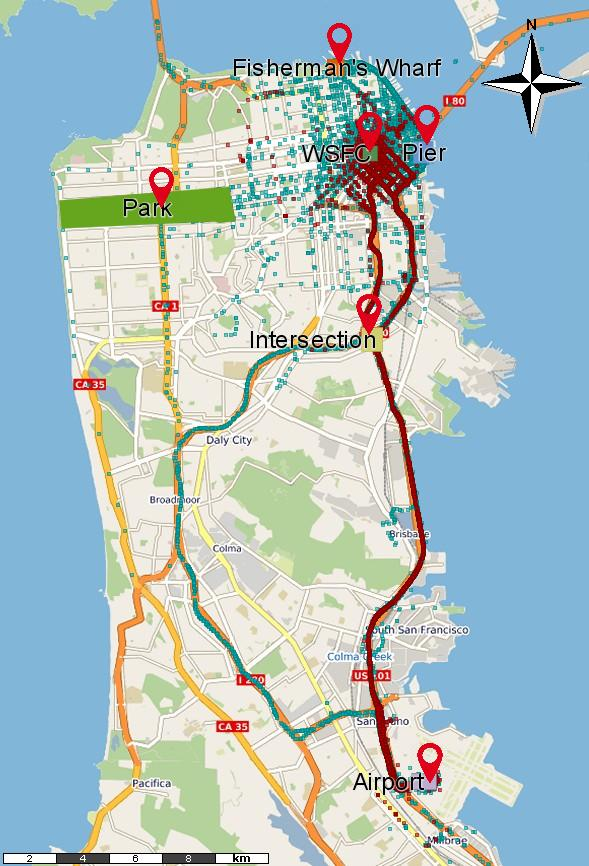
\includegraphics[width=.45\textwidth]{Images/new_CRAWDAD-Trajectories-Painted}
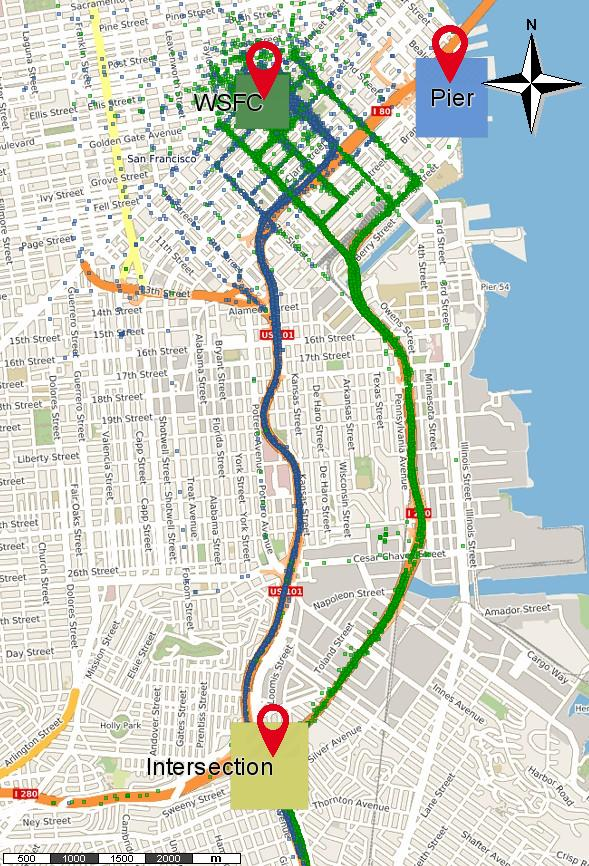
\includegraphics[width=.45\textwidth]{Images/new_CRAWDAD-Paths-Painted}
\caption{\hl{The map at left shows the taxi trajectories moving between the six regions, where red points are the interested trajectories and light blue points are the no interested trajectories. The map at right shows the interested trajectories, where dark blue points are the trajectories moving on highway 101 and green points are trajectories using highway 280}}
\label{fig:new_sanfrancisco_map_rois}
\end{figure}

\hl{With the objective of characterizing the trajectory movement, we separate the interested trajectories based on which region and road was followed, whether 101 or 280, two major roads connecting the Airport to downtown. Figure {\ref{fig:new_sanfrancisco_map_rois}} (right) presents a zoom over trajectories moving between the \textbf{Airport} region and the \textbf{WSFC} region using the \textbf{Intersection} of highways 101 (blue) and 280 (green), where we can clearly visualize that the trajectories have different \emph{moves}.

Considering the stops WSFC, Intersection, and Airport, we consider as the ground truth the four distinct paths followed by the trajectories that move between these regions. These paths are shown in Table {\ref{tab:new_san_francisco_dataset}}. All 60 trajectories moving from Airport in direction to WSFC via highway 101 are defined as class A1. The 619 trajectories moving in opposite direction from WSFC to the Airport by highway 101 belong to class A2. The 232 trajectories moving from Airport in direction to WSFC by highway 280 belong to class B1 and the 374 trajectories moving from WSFC in direction to Airport by highway 280 belong to class B2. We assume that trajectories that belong to the same class should be more similar than trajectories of different classes.}

\begin{table}[h]
\scriptsize
  \centering
  \begin{tabular}{|c|c|c|c|c|}
  	\hline
 Direction & Highway & Trajectories & Class \\
  	\hline
 Airport to WSFC & 101 & 60 & A1\\
 WSFC to Airport & 101 & 619 & A2\\
 Airport to WSFC & 280 & 232 & B1\\
 WSFC to Airport & 280 & 374 & B2\\
    \hline
  \end{tabular}
  \caption{Summary of interested trajectories extracted from the taxi trajectories dataset}
  \label{tab:new_san_francisco_dataset}
\end{table}

\subsubsection{Results for the taxi trajectories}

\hl{In this experiment we considered the following dimensions for stops and moves: as spatial dimension of the stops we considered the centroid of the stop; as temporal dimension we used both start and end time of the stop; and as semantic information we used the name of the region (WSFC, Pier, Fisherman's Wharf, Park, Intersection, and Airport). For the moves we analyze the real movement, and use as spatial dimension the moves raw points.}

\hl{For measuring the stop similarity we use: (i) the Euclidean distance for space; (ii)for the semantics, the distance is 0 in case of exact match and 1 otherwise; and (iii) for the time dimension, where $[t1, t2]$ is the time interval of a stop, the time distance of two stops is given by  Equation {\ref{func:time_interval}}.

For the moves, we consider the raw trajectory points and use UMS, because it is appropriate for low sampled trajectories, which is the case for this dataset.

In this experiment we consider the same weights for each dimension and for stops and moves, so 0.5 for the stops and 0.5 for the moves, and 0.33 for space, time, and semantics. Later in the parameter analysis section we show how the results change as we vary the weights of the stops and moves, as they are the central contribution of this paper.

As several measures were not developed for semantic trajectories, for a more fair comparison we apply existing measures over semantic trajectories and over raw trajectories. For doing so we split the experiment in two parts: 1) a \textit{precision at recall} evaluation using only semantic trajectories; and 2) a \textit{precision at recall} evaluation using the raw trajectories.}

\hl{Table {\ref{tab:new_san_francisco_measures}} summarizes the dimensions used in each measure. To general multidimensional similarity measures as MSM, we provide as input all dimensions of each stop, namely: 1) spatial information; 2) time interval; and 3) semantic information. We extend LCSS and EDR to support multiple dimensions, using the same strategy used in }\cite{Furtado:TGIS12156}\hl{: given two multidimensional trajectories, two points are said as matched when all dimensions match, where each dimension has a distinct distance threshold. With those adaptations, both LCSS and EDR are used to measure similarity using the dimensions of space, time and semantics for stops. For CVTI, we provide as input the time interval of the stops and the stop names. For MSTP, we provide the stop names only.}

\begin{table}[!h]
\scriptsize
  \centering
  \begin{tabular}{|l|c|c|c|c|c|}
  	\hline
  & \multicolumn{4}{c|}{Semantic trajectories} & \multicolumn{1}{c|}{Raw trajectories} \\
 	\cline{2-5}
  & \multicolumn{3}{c|}{Stop} & \multicolumn{1}{c|}{Move} & \multicolumn{1}{c|}{} \\
 	\cline{2-6}
  & Space & Time & Semantics & Trajectory points & Space\\
  	\hline
 SMSM & X & X & X & X & \\
 MSM & X & X & X & &\\
 MSTP &  &  & X & & \\
 CVTI & & X & X & & \\
 LCSS & X & X & X & & X \\
 EDR & X & X & X & & X \\
 DTWa &  &  &  & & X \\
 UMS & & & & & X \\
 wDF & & & & & X \\
    \hline
  \end{tabular}
  \caption{Dimensions used for each measure}
  \label{tab:new_san_francisco_measures}
\end{table}

\hl{Table {\ref{tab:new_san_francisco_thresholds}} shows the  thresholds used for each measure. To define threshold values for the stops we experimented  a range of values on each dimension as follows: for space (distance between stop centroids) we varied the distance from 100m to 500m in a 100 meters range; and for the time distance we tested a proportion of intersection from 0\% to 100\% varying in ranges of 10 \%. For the move threshold we varied the UMS similarity for two moves from 0 to 1 in a 0.1 unit step.

Table {\ref{tab:new_sanfrancisco_measures_map_auc}} shows the comparison of SMSM with approaches developed either for raw or semantic trajectories.
For semantic trajectories, SMSM (MAP=0.67) outperformed the other measures in at least 45 \%. This occurs because state-of-the-art measures do not take into account the move between two stops.
For raw trajectories, DTWa (MAP=0.47) was the second most accurate measure and UMS (MAP=0.37) was third most accurate measure. This is an expected result since the proposed experiment is strongly based on spatial dimension. Despite of that, SMSM outperforms all kind of similarity measures since it takes into account both the order of \emph{stops} and the \emph{move} between the \emph{stops}.}

\begin{table}[!h]
\scriptsize
  \centering
  \begin{tabular}{|c|c|c|c|c|}
  	\hline
  & \multicolumn{3}{c|}{Semantic trajectories} & \multicolumn{1}{c|}{Raw trajectories} \\
 	\cline{2-5}
  & Space (meters) & Time proportion & Move & Space (meters) \\
  	\hline
 SMSM & 100 & 0.3 & 0.8 & - \\
 MSM & 100 & 0.1 & - & - \\
 LCSS & 100 & 0.1 & - & 100 \\
 EDR & 100 & 0.1 & - & 100 \\
    \hline
  \end{tabular}
  \caption{Thresholds used for each measure}
  \label{tab:new_san_francisco_thresholds}
\end{table}


\begin{table}[h]
\scriptsize
  \centering
  \begin{tabular}{|l|c|c|c|c|}
  	\hline
 & \multicolumn{2}{c}{Semantic} & \multicolumn{2}{|c|}{Raw} \\
 	\cline{2-5}
 & MAP & AUC & MAP & AUC \\
  	\hline
SMSM & \textbf{0.70} & \textbf{0.74} & - & -\\
DTWa & - & - & 0.47 & 0.51 \\
UMS & - & - & 0.37 & 0.41 \\
MSM & 0.36 & 0.39 & - & - \\
wDF & - & - & 0.32 & 0.36 \\
MSTP & 0.27 & 0.31 & - & - \\
EDR & 0.26 & 0.30 & 0.29 & 0.33 \\
LCSS & 0.26 & 0.30 & 0.27 & 0.31 \\
CVTI & 0.24 & 0.29 & - & - \\
    \hline
  \end{tabular}
  \caption{MAP and AUC evaluation for the \hl{taxi} dataset}
  \label{tab:new_sanfrancisco_measures_map_auc}
\end{table}


\hl{Figure {\ref{fig:new_sanfrancisco_precision_recall}} (left) shows the \emph{precision at recall} graph for semantic trajectories. As can be seen, SMSM was better to recover trajectories of the same class than the other methods in almost all recall levels. All other measures were much worse than SMSM, having a precision at least 45\% lower than SMSM. It happens because these measures do not consider the moves and the order of stops.}


\begin{figure*}[ht!]
\centering
\centerline{
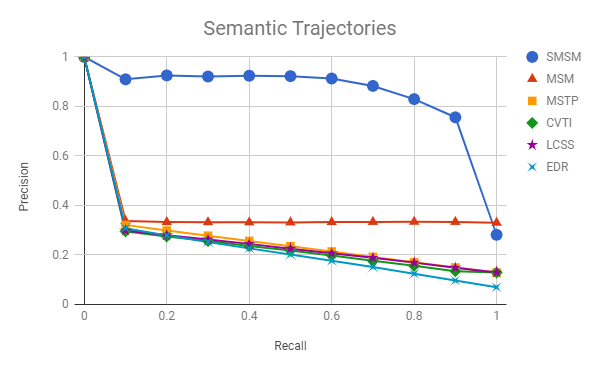
\includegraphics[width=0.5\textwidth]{Images/new_P_R-chart_San_Francisco.png}
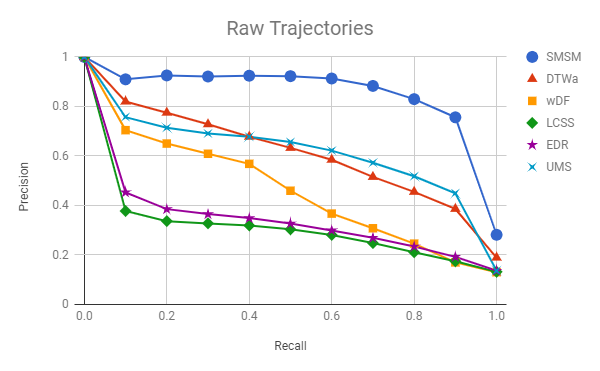
\includegraphics[width=0.5\textwidth]{Images/new_P_R-chart_San_Francisco-raw.png}
}
\caption{ Precision at recall results for semantic and raw trajectories}
\label{fig:new_sanfrancisco_precision_recall}
\end{figure*}



\hl{Figure {\ref{fig:new_sanfrancisco_precision_recall}} (right) shows the \emph{precision at recall} of measures for raw trajectories, which performed better than the measures for semantic trajectories in this dataset. This occurs because the defined classes are very related to spatial movement of the taxi. But SMSM still obtained a better score. The second best measure was DTWa. UMS was the third better measure. This happens because the dynamic ellipses do better capture the raw point distances over varying sampling rates.
All remaining measures performed worse because they all use a fixed threshold to define spatial matching between the points.}

\begin{comment}
%Antigo experimento do CRAWDAD
\subsection{Experiment with the \hl{taxi} dataset}\label{sec:crawdad}

The \hl{epfl/mobility} dataset contains taxi trips in San Francisco collected between May and June 2008, with an average sampling rate of about one point per minute. Each trajectory has several days of duration, what is not useful to determine similar movements around the town. For that reason, we split each taxi trajectory into short trajectories, (i) splitting when the occupation status of the taxi changed (taken or free) and (ii) splitting when a 5 minutes gap between two consecutive points was found.

\subsubsection{Ground truth generation}
In order to evaluate SMSM we generated a ground truth dataset, since there is no real trajectory dataset with stops and moves to evaluate trajectory similarity. For this purpose, we selected three distinct regions in San Francisco with high density of trajectories, that we have considered as the stops. These regions are shown in Figure \ref{fig:sanfrancisco_map_rois}(left), and are the Westfield San Francisco Center (\textbf{WSFC}), the \textbf{Intersection} between highways 280 and 101, and San Francisco \textbf{Airport}. 

\begin{figure}[ht!]
\centering
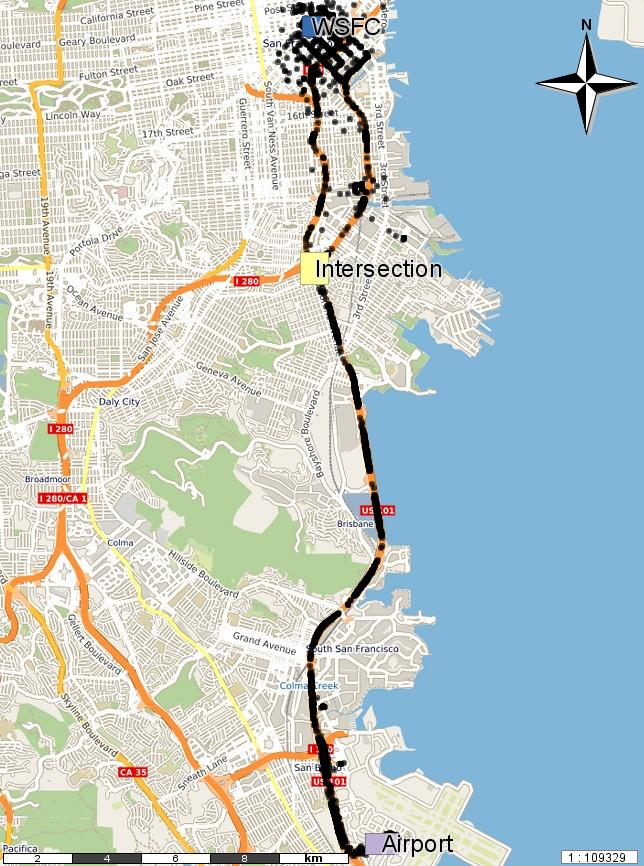
\includegraphics[width=.49\textwidth]{Images/CRAWDAD-Trajectories-Painted}
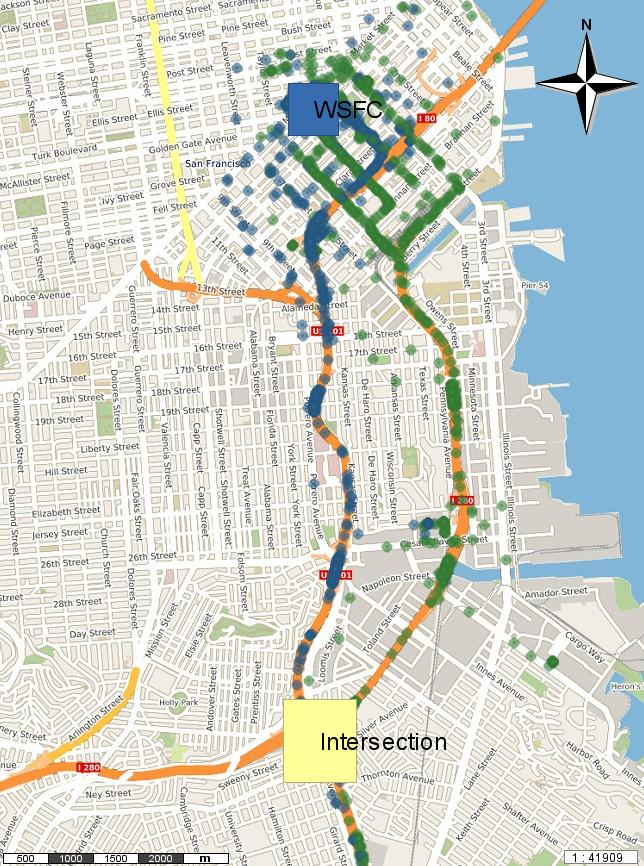
\includegraphics[width=.49\textwidth]{Images/CRAWDAD-Paths-Painted}
\caption{(left) \hl{taxi} trajectories moving from Airport to WSFC and vice-versa (right) \hl{taxi trajectories represented with different colors, where blue points are the trajectories moving on highway 101 and green points are trajectories using highway 280}}
\label{fig:sanfrancisco_map_rois}
\end{figure}

With the objective of characterizing the trajectory movement, we separate the trajectories based on which road was followed, whether 101 or 280, two major roads \hl{connecting the Airport to} WSFC. {Figure \ref{fig:sanfrancisco_map_rois}} (right) presents a zoom over trajectories moving on highways 101 (blue) and 280 (green) from Intersection to WSFC, where we can clearly visualize that the trajectories have different \emph{moves}.

Considering the stops WSFC, Intersection, and Airport, we consider as the ground truth the four distinct paths followed by the trajectories that move between these regions. These paths are shown in Table \ref{tab:san_francisco_dataset}. All 25 trajectories moving from Airport in direction to WSFC via highway 101 are defined as class A1. The 101 trajectories moving in opposite direction from WSFC to the Airport by highway 101 belong to class A2. The 34 trajectories moving from Airport in direction to WSFC by highway 280 belong to class B1 and the 44 trajectories moving from WSFC in direction to Airport by highway 280 belong to class B2. We assume that trajectories that belong to the same class should be more similar than trajectories of different classes.

\begin{table}[h]
\scriptsize
  \centering
  \begin{tabular}{|c|c|c|c|c|}
  	\hline
 Direction & Highway & Trajectories & Class \\
  	\hline
 Airport to WSFC & 101 & 25 & A1\\
 WSFC to Airport & 101 & 101 & A2\\
 Airport to WSFC & 280 & 34 & B1\\
 WSFC to Airport & 280 & 44 & B2\\
    \hline
  \end{tabular}
  \caption{Summary of trajectories extracted from the taxi trajectories dataset}
  \label{tab:san_francisco_dataset}
\end{table}

\subsubsection{Results for the taxi trajectories}

In this experiment we considered the following dimensions for stops and moves: as spatial dimension of the stops we considered the centroid of the stop; as temporal dimension we used both start and end time of the stop; and as semantic information we used the name of the region (Airport, Intersection, and WSFC). For the moves we analyze the real movement, and use as spatial dimension the moves raw points.

For measuring the stop similarity we use: (i) the Euclidean distance for space; (ii)\hl{ for the semantics, the distance is 0 in case of exact match and 1 otherwise; and (iii) for the time dimension, where $[t1, t2]$ is the time interval of a stop, the time distance of two stops is given by  Equation} \ref{func:time_interval}.




For the moves, we consider the raw trajectory points and use UMS, because it is appropriate for low sampled trajectories, which is the case for this dataset. %, and it outperformed all existing similarity measures for raw trajectories evaluated in \cite{Furtado-UMS-2018}.

\hl{In this experiment we consider the same weights for each dimension and for stops and moves, so 0.5 for the stops and 0.5 for the moves, and 0.33 for space, time, and semantics. Later in the parameter analysis section we show how the results change as we vary the weights of the stops and moves, as they are the central contribution of this paper.}

As several measures were not developed for semantic trajectories, for a more fair comparison we apply existing measures over semantic trajectories and over raw trajectories. For doing so we split the experiment in two parts: 1) a \textit{precision at recall} evaluation using only semantic trajectories; and 2) a \textit{precision at recall} evaluation using the raw trajectories.% In (1) we run the experiment using the following measures: SMSM, MSM, MSTP, CVTI, LCSS and EDR. In (2) we run the experiment for the following measures: DTWa, wDF, LCSS, EDR and UMS.

Table {\ref{tab:san_francisco_measures}} summarizes the dimensions used in each measure. To general multidimensional similarity measures as MSM, we provide as input all dimensions of each stop, namely: 1) spatial information; 2) time interval; and 3) semantic information. We extend LCSS and EDR to support multiple dimensions, using the same strategy used in {\cite{Furtado:TGIS12156}}: given two multidimensional trajectories, two points are said as matched when all dimensions match, where each dimension has a distinct distance threshold. With those adaptations, both LCSS and EDR are used to measure similarity using the dimensions of space, time and semantics for stops. For CVTI, we provide as input the time interval of the stops and the stop names. \hl{For MSTP, we provide the stop names only.}

\begin{table}[!h]
\scriptsize
  \centering
  \begin{tabular}{|l|c|c|c|c|c|}
  	\hline
  & \multicolumn{4}{c|}{Semantic trajectories} & \multicolumn{1}{c|}{Raw trajectories} \\
 	\cline{2-5}
  & \multicolumn{3}{c|}{Stop} & \multicolumn{1}{c|}{Move} & \multicolumn{1}{c|}{} \\
 	\cline{2-6}
  & Space & Time & Semantics & Trajectory points & Space\\
  	\hline
 SMSM & X & X & X & X & \\
 MSM & X & X & X & &\\
 MSTP &  &  & X & & \\
 CVTI & & X & X & & \\
 LCSS & X & X & X & & X \\
 EDR & X & X & X & & X \\
 DTWa &  &  &  & & X \\
 UMS & & & & & X \\
 wDF & & & & & X \\
    \hline
  \end{tabular}
  \caption{Dimensions used for each measure}
  \label{tab:san_francisco_measures}
\end{table}

Table \ref{tab:san_francisco_thresholds} shows the  thresholds used for each measure. To define threshold values for the stops we experimented  a range of values on each dimension as follows: for space (distance between stop centroids) we varied the distance from 100m to 500m in a 100 meters range; and for the time distance we tested a proportion of intersection from 0\% to 100\% varying in ranges of 10 \%. For the move threshold we varied the UMS similarity for two moves from 0 to 1 in a 0.1 unit step.

\hl{Table {\ref{tab:sanfrancisco_measures_map_auc}} shows the comparison of SMSM with approaches developed either for raw or semantic trajectories.
For semantic trajectories, SMSM (MAP=0.92) outperformed the other measures in more than 50 \%. This occurs because state-of-the-art measures do not take into account the move between two stops.} \textcolor{Red}{nao estou convencida de todos darem o mesmo resultado, inclusive o UMS e DTWa. Precisa justificar isso porque eu nao compreendo. MSTP e CVTI tambem?}
\hl{For raw trajectories, DTWa and UMS (MAP=0.89) were very accurate, since the proposed experiment is strongly based on spatial dimension. Despite of that, SMSM outperforms all kind of similarity measures since it takes into account both the order of \emph{stops} and the \emph{move} between the \emph{stops}.}
%, because although developed for raw trajectories, in this dataset the stops and moves of all trajectories are very similar. UMS has a good performance because it captures the trajectories that follow the same roads and their direction.

\begin{table}[!h]
\scriptsize
  \centering
  \begin{tabular}{|c|c|c|c|c|}
  	\hline
  & \multicolumn{3}{c|}{Semantic trajectories} & \multicolumn{1}{c|}{Raw trajectories} \\
 	\cline{2-5}
  & Space (meters) & Time proportion & Move & Space (meters) \\
  	\hline
 SMSM & 100 & 0.3 & 0.9 & - \\
 MSM & 100 & 0.3 & - & - \\
 LCSS & 100 & 0.3 & - & 100 \\
 EDR & 100 & 0.3 & - & 100 \\
    \hline
  \end{tabular}
  \caption{Thresholds used for each measure}
  \label{tab:san_francisco_thresholds}
\end{table}


\begin{table}[h]
\scriptsize
  \centering
  \begin{tabular}{|l|c|c|c|c|}
  	\hline
 & \multicolumn{2}{c}{Semantic} & \multicolumn{2}{|c|}{Raw} \\
 	\cline{2-5}
 & MAP & AUC & MAP & AUC \\
  	\hline
SMSM & \textbf{0.92} & \textbf{0.93} & - & -\\
UMS & - & - & 0.89 & 0.91 \\
DTWa & - & - & 0.89 & 0.91 \\
LCSS & 0.41 & 0.44 & 0.83 & 0.85 \\
EDR & 0.41 & 0.44 & 0.82 & 0.84 \\
wDF & - & - & 0.65 & 0.68 \\
MSM & 0.41 & 0.44 & - & - \\
MSTP & 0.41 & 0.44 & - & - \\
CVTI & 0.41 & 0.44 & - & - \\
    \hline
  \end{tabular}
  \caption{MAP and AUC evaluation for the \hl{taxi} dataset}
  \label{tab:sanfrancisco_measures_map_auc}
\end{table}

%\begin{table}[h]
%\scriptsize
%  \centering
%  \begin{tabular}{|l|c|c|c|c|}
%  	\hline
% & \multicolumn{2}{c}{Semantic} & \multicolumn{2}{|c|}{Raw} \\
% 	\cline{2-5}
% & MAP & AUC & MAP & AUC \\
%  	\hline
%SMSM & \textbf{0.98} & \textbf{0.98} & - & -\\
%UMS & - & - & 0.92 & 0.93 \\
%DTWa & - & - & 0.84 & 0.87\\
%wDF & - & - & 0.73 & 0.75\\
%EDR & 0.72 & 0.74 & 0.64 & 0.66\\
%LCSS & 0.65 & 0.67 & 0.55 & 0.57\\
%MSM & 0.57 & 0.60 & - & -\\
%MSTP & 0.56 & 0.60 & - & -\\
%CVTI & 0.55 & 0.58 & - & -\\
%    \hline
%  \end{tabular}
%  \caption{(old results) MAP and AUC evaluation for the \hl{taxi} dataset}
%  \label{tab:sanfrancisco_measures_map_auc_antigo}
%\end{table}

\hl{Figure {\ref{fig:sanfrancisco_precision_recall}} (left) shows the \emph{precision at recall} graph for semantic trajectories. As can be seen, SMSM was better to recover trajectories of the same class than the other methods in all recall levels. All other measures were much worse than SMSM, having a precision around 55\% lower than SMSM. It happens because these measures do not consider the moves and the order of stops.}
%MSM also does not handle heterogeneous data and it does not take the sequence of elements into account. This explains the worse MSM results, since the measure ignores the \emph{move} between \emph{stops} and the sequence of \emph{stops}. CVTI and MSTP, despite of being LCSS-based measures, have the worst results because the measures do not take into account some information, such as geospatial data in CVTI, or the use of only the frequency of the \emph{stops}, as MSTP.}

\begin{figure*}[ht!]
\centering
\centerline{
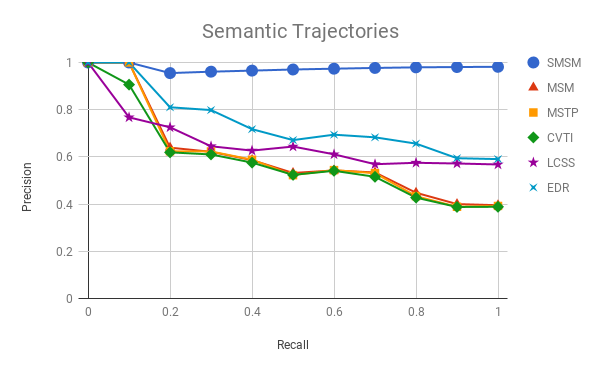
\includegraphics[width=0.5\textwidth]{Images/P_R-chart_San_Francisco.png}
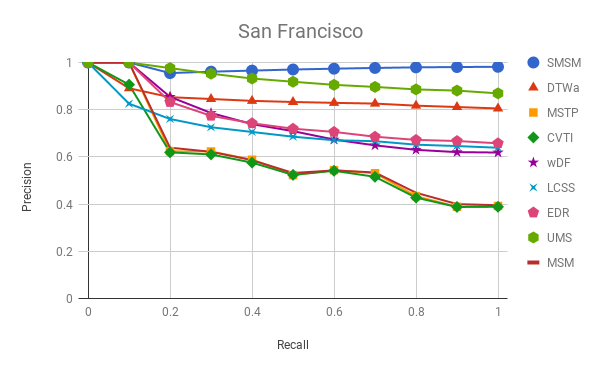
\includegraphics[width=0.5\textwidth]{Images/P_R-chart_San_Francisco-raw.png}
}
\caption{ Precision at recall results for semantic and raw trajectories}
\label{fig:sanfrancisco_precision_recall}
\end{figure*}



\hl{Figure {\ref{fig:sanfrancisco_precision_recall}} (right) shows the \emph{precision at recall} of measures for raw trajectories, which performed better than the measures for semantic trajectories in this dataset. This occurs because the defined classes are very related to spatial movement of the taxi. But SMSM still obtained a better score. The second best measure was UMS, because the ellipses do better capture the raw point distances over varying sampling rates. The third most accurate measure was DTWa.  
%DTWa tries to minimize the overall distance between two raw trajectories and the GPS points help the measure to correctly recover the trajectories of the same class. 
All remaining measures, except wDF, performed well.
% EDR and LCSS measures, although originally developed for raw trajectories had bad results because of the point-by-point analysis, where they make the point match only when the distance of two points is less than a threshold, so the smaller the sampling rate, the more difficult to give a match. wDF also compares trajectories point-by-point, but its \emph{window} parameter allows it to minimize the impact of low sampled trajectories. Therefore, wDF had better results than LCSS and EDR even being a point-to-point measure. In summary, SMSM results with semantic trajectories were better than all other raw similarity measures.
}
\end{comment}

\subsection{Experiment with the Geolife Dataset}\label{sec:geolife}

The Geolife is a well-known trajectory dataset, created by Microsoft Research Asia \citep{zheng2009mining} containing trajectories of 182 users, moving around Beijing, collected between April 2007 and August 2012. As a preprocessing step, we split trajectories when a 5 minutes gap between two consecutive points was found, since the trajectories of this dataset are highly sampled (lower than 2s).

\begin{figure}[ht!]
\centering
\centerline{
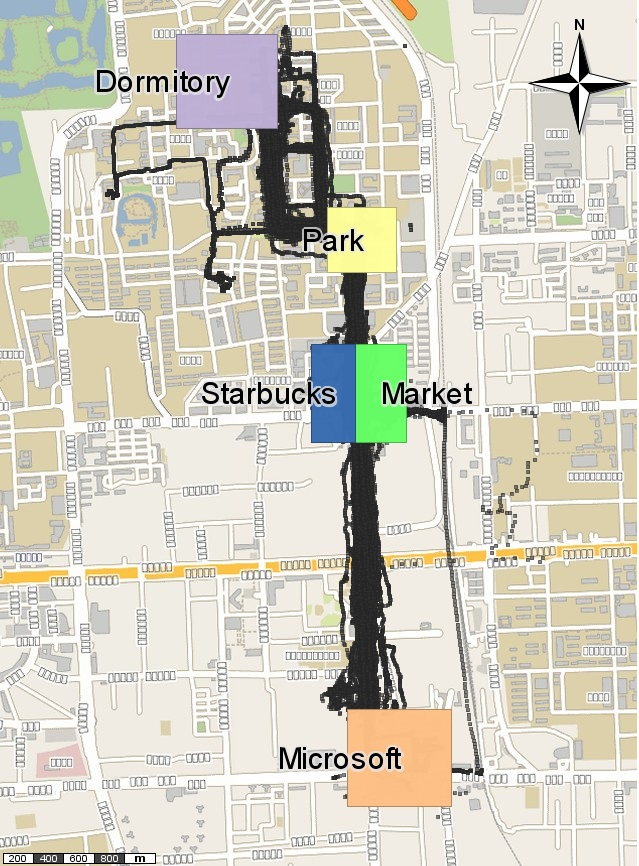
\includegraphics[width=.5\textwidth]{Images/Geolife-Trajectories-painted.jpg}
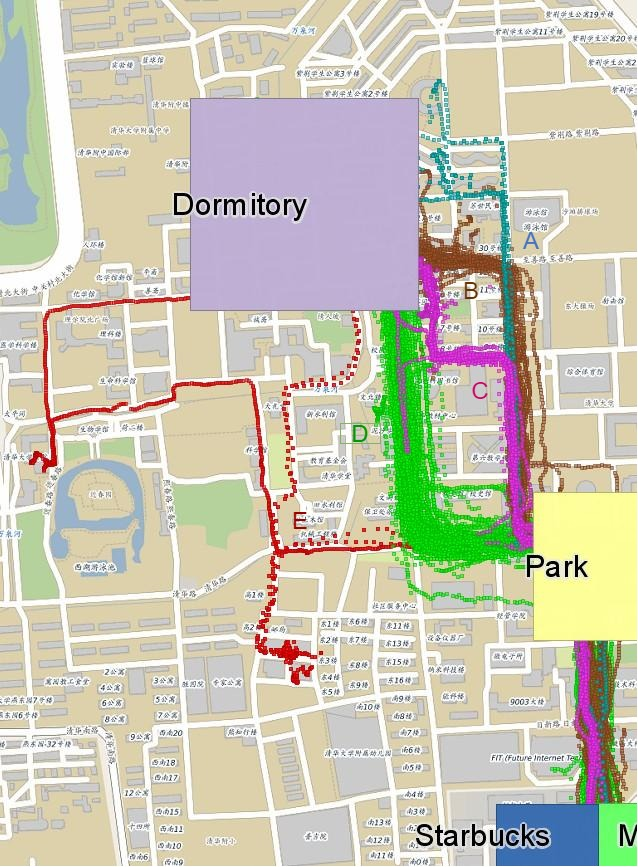
\includegraphics[width=.5\textwidth]{Images/Geolife-Paths-painted.jpg}
}
\caption{(left) trajectories moving between the regions Microsoft, Starbucks, Market, Park, and Dormitory (right) zoom over the distinct moves performed between Park and Dormitory}
\label{fig:geolife_map_rois}
\end{figure}

\subsubsection{Ground Truth Definition}
\hl{As the Geolife dataset has no ground truth for evaluating similarity measures, we had to generate a ground truth. We had to find stops where the objects make different moves between the stops in order to distinguish the trajectories.}
To build the ground truth, we chose an area in Beijing, where pedestrians move between the University Dormitories and Microsoft Research Office. We considered five places as stops (Microsoft, Starbucks, Market, Park and Dormitory), that are show in Figure \ref{fig:geolife_map_rois} (left). We considered 5 distinct paths connecting the stops, labeled as A, B, C, D, and E, as shown in Figure \ref{fig:geolife_map_rois} (right).

In Table \ref{tab:geolife_dataset} we define as ground truth 8 distinct classes of movement based on the sequence of stops and the followed path: Microsoft to Dormitory via Market and Park by path A with 5 trajectories named as class A, Microsoft to Dormitory via Market and Park by path B with 40 trajectories named as class B, Dormitory to Microsoft via Park and Starbucks by path C with 11 trajectories named as class C, Dormitory to Microsoft via Park and Starbucks by path D with 115 trajectories named as class D1, Dormitory to Microsoft via Park and Market by path D with 7 trajectories named as class D2, Microsoft to Dormitory via Market and Park by path D with 149 trajectories named as class D3, Microsoft to Dormitory via Starbucks and Park by path D with 6 trajectories named as class D4 and Microsoft to Dormitory via Market and Park by path E with 4 trajectories named as class E.

\begin{table}[ht!]
\scriptsize
  \centering
  \begin{tabular}{|c|c|c|c|}
  	\hline
 Direction & Path &  Trajectories & Class \\
  	\hline
Microsoft to Dormitory via Market and Park& A & 5 & A \\
Microsoft to Dormitory via Market and Park& B & 40&B \\
Dormitory to Microsoft via Park and Starbucks& C & 11&C \\
Dormitory to Microsoft via Park and Starbucks& D & 115&D1 \\
Dormitory to Microsoft via Park and Market& D & 7&D2 \\
Microsoft to Dormitory via Market and Park& D & 149&D3 \\
Microsoft to Dormitory via Starbucks and Park& D & 6&D4 \\
Microsoft to Dormitory via Market and Park& E & 4& E \\
    \hline
  \end{tabular}
  \caption{Classes representing distinct paths for the ground truth}
  \label{tab:geolife_dataset}
\end{table}

\subsubsection{Results with the Geolife dataset}

Following a similar methodology used for the previous experiment, we calculate the precision at recall for all 8 classes in our ground truth, comparing the SMSM results to the other measures. The dimensions used for stops are: a) space; and b) the region name (Dormitory, Park, Starbucks, Market and Microsoft). For the moves we used the raw points of the move. The time dimension was not taken into account because in this experiment we have classes with a few trajectories and most of them do not match in time.

For measuring the stop similarity we use: (i) the Euclidean distance for space; and (ii) 1 and 0 for the semantics in case of exact match or no match, respectively. For the moves,  we consider the raw trajectory points. In this experiment we use DTW distance for analyzing the spatial similarity of the moves, because the trajectory points are highly sampled \hl{and trajectory points are very near in space}. %, and UMS is not a good measure when points are highly sampled as in the Geolife dataset, so not distinguishing the different paths.
For this dataset UMS is not good for distinguishing the moves\hl{, since it was developed for irregular sampling}.

\hl{For the weight, we use 0.5 for stops and 0.5 for moves, giving the same importance, and for the dimensions, we use 0.5 for space and 0.5 for semantics.}

Table \ref{tab:geolife_thresholds} presents the thresholds used for each measure. We defined the thresholds by running each experiment over a range of possible threshold values and the best results for each method were reported. For raw trajectories, we evaluated as threshold the  values 2, 4, 6, 8 and 10 meters because this dataset is highly sampled and is of pedestrian trajectories. The threshold for the move dimension was defined as follows: two moves are said to match if the DTW distance between them is less than the sum of the Euclidean distance of the moves.

\begin{table}[!h]
\scriptsize
  \centering
  \begin{tabular}{|c|c|c|}
  	\hline
  & \multicolumn{1}{c|}{Semantic trajectories} & \multicolumn{1}{c|}{Raw trajectories} \\
 	\cline{2-3}
  & Space (meters) & Space (meters) \\
  	\hline
 SMSM & 100 & - \\
 MSM & 100 & - \\
 LCSS & 100 & 8 \\
 EDR & 100 & 8 \\
    \hline
  \end{tabular}
  \caption{Thresholds used for each measure}
  \label{tab:geolife_thresholds}
\end{table}

Table \ref{tab:geolife_measures_map_auc} shows the experimental results. As can be observed in the table\hl{, SMSM outperforms all measures for semantic trajectories, being significantly better than MSM, that ignores the moves and the sequence. LCSS and EDR perform better than MSM because the order of the stops is important. The measures for raw trajectories perform well in this dataset because the raw trajectories of the dataset discriminate the class.}
%Table \ref{tab:geolife_measures_map_auc} shows the experimental results. As can be observed in the table, SMSM outperforms all other measures for raw or semantic trajectories. SMSM was significantly better than MSM, LCSS, and EDR over semantic trajectories. \hl{For this dataset, DTWa, LCSS, and EDR performed well over raw trajectories, but still the MAP score of SMSM (0.95) using only the semantic trajectories was greater than other measures.}

%The 1st and 2nd columns of Table \ref{tab:geolife_measures_map_auc} show that SMSM results for MAP and AUC (0.95/0.95) were higher than MSM, LCSS, EDR (0.74/0.75), CVTI (0.53/0.57), and MSTP (0.50/0.53). The bad results of all other measures show that the moves discriminate the trajectories, since any other measures does not consider the moves. For semantic trajectories MSM, LCSS, and EDR perform very similarly. %In addition, executing the experiment using raw trajectories (3rd and 4rd columns in Table \ref{tab:geolife_measures_map_auc}), the results of DTWa (0.86/0.87), UMS (0.84/0.85), LCSS (0.79/0.80), EDR (0.71/0.73), and wDF (0.57/0.60) did not reach the good results of SMSM.

\begin{table}[ht!]
  \scriptsize
  \centering
  \begin{tabular}{|l|c|c|c|c|}
  	\hline
 & \multicolumn{2}{c}{Semantic}& \multicolumn{2}{|c|}{Raw}\\
 	\cline{2-5}
 & MAP & AUC & MAP & AUC\\
  	\hline
SMSM & \textbf{0.95} & \textbf{0.96} & - & -\\
DTWa & - & - & 0.93 & 0.94\\
LCSS & 0.74 & 0.75 & 0.82 & 0.84\\
 EDR & 0.74 & 0.75 & 0.81 & 0.84\\
 UMS & - & - & 0.70 & 0.73\\
 MSM & 0.69 & 0.71 & - & -\\
 wDF & - & - & 0.58 & 0.61\\
CVTI & 0.43 & 0.46 & - & -\\
MSTP & 0.41 & 0.44 & - & -\\
    \hline
  \end{tabular}
  \caption{MAP and AUC evaluation for the experiment with the Geolife dataset}
  \label{tab:geolife_measures_map_auc}
\end{table}

%\begin{table}[ht!]
%  \scriptsize
%  \centering
%  \begin{tabular}{|l|c|c|c|c|}
%  	\hline
% & \multicolumn{2}{c}{Semantic}& \multicolumn{2}{|c|}{Raw}\\
% 	\cline{2-5}
% & MAP & AUC & MAP & AUC\\
%  	\hline
%SMSM & \textbf{0.95} & \textbf{0.95} & - & -\\
%DTWa & - & - & 0.86 & 0.87\\
%LCSS & 0.74 & 0.75 & 0.85 & 0.86\\
% UMS & - & - & 0.84 & 0.85\\
% EDR & 0.74 & 0.75 & 0.71 & 0.73\\
% MSM & 0.74 & 0.75 & - & -\\
% wDF & - & - & 0.57 & 0.60\\
%CVTI & 0.53 & 0.57 & - & -\\
%MSTP & 0.50 & 0.53 & - & -\\
%    \hline
%  \end{tabular}
%  \caption{(old results) MAP and AUC evaluation for the experiment with the Geolife dataset}
%  \label{tab:geolife_measures_map_auc_antigo}
%\end{table}


\hl{Figure {\ref{fig:geolife_precision_recall}} shows the precision at recall results. Figure {\ref{fig:geolife_precision_recall}} (left) shows that SMSM was better to recover semantic trajectories of the same class in all recall levels. LCSS, EDR and MSM had the same results because they do not take into account the moves. Figure {\ref{fig:geolife_precision_recall}} (right) shows that all measures, except wDF, performed well, but SMSM is better to recover trajectories of same class in almost all recall levels.}
%\hl{Figure {\ref{fig:geolife_precision_recall}} shows the precision at recall levels, where SMSM had the best results over all other measures developed for either semantic (left) or raw (right) trajectories. Figure {\ref{fig:geolife_precision_recall}} (left)  shows that SMSM was better to recover semantic trajectories of the same class in almost all recall levels. LCSS and EDR had worse results than SMSM because these measures do not take into account the \emph{move} element between the \emph{stops}. The results were not worst because the measures take into account the sequence of \emph{stops}. Even without considering both the \emph{moves} and the sequence of \emph{stops}, MSM had a similar precision at recall curve. This occurs because spatial and semantics values of the \emph{stops} are strongly related (e.g. all \emph{stops} of Dormitory POI have same spatial coordinate). If the \emph{stops} occur in distinct spatial locations, but remaining the POI name, MSM would score as similar two \emph{stops} spatially near, but semantically distinct, affecting the precision at recall results. MSTP and CVTI, as LCSS-based measures with constraints, have the same problems of the taxi experiment: i) CVTI does not take into account the spatial dimension, and in this dataset the semantic dimension are closely related to spatial dimension; and ii) MSTP makes use of the frequency of the \emph{stops}, and all trajectories in this dataset are short and non-repetitive trajectories, demanding the measure to use only the spatial data of each \emph{stop}. Figure {\ref{fig:geolife_precision_recall}} (right) shows that all measures, except wDF performed well, but SMSM is better to recover trajectories of same class in all recall levels. }

\begin{figure*}[ht!]
\centerline{
\centering
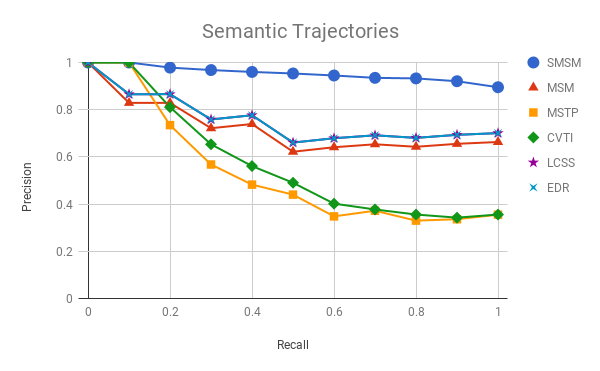
\includegraphics[width=.55\textwidth]{Images/P_R-chart_Geolife.png}
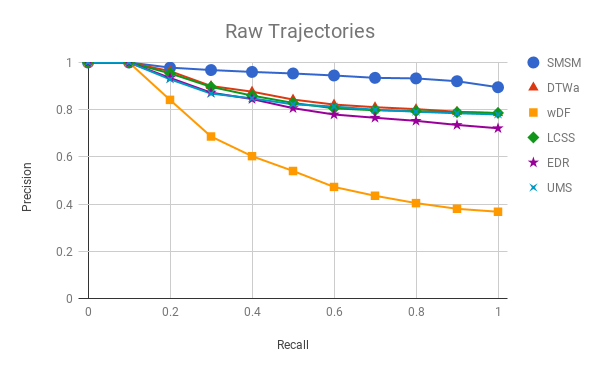
\includegraphics[width=.55\textwidth]{Images/P_R-chart_Geolife-raw.png}
}
\caption{Precision at recall results to semantic (left) and raw (right) trajectories}
\label{fig:geolife_precision_recall}
\end{figure*}
%We notice that, in general, all similarity measures have a good result. However, we observed from the similarity scores shown in Table \ref{tab:geolife_similaritymeans} that some measures having a high precision at recall, give a low similarity degree for trajectories of the same class that are highly similar. So to compare how well a measure can identify very similar trajectories of the same class, we perform another analysis: we extracted the mean similarity scores by class for each measure. We expect all trajectories of the same class to be more similar between them, with higher similarity scores.
%Table \ref{tab:geolife_similaritymeans} shows the mean similarity scores by class for each measure. For each measure, we choose the best AUC score, either from the semantic or raw trajectory results. The best results by class are in bold and the second better results are in italic. The results clearly show that the similarity score between trajectories of the same class is greater using SMSM than all others measures. The other two better measures in this analysis are MSM and DTWa. LCSS, for instance, had a good result in precision at recall in Table \ref{tab:geolife_measures_map_auc}, but the average similarity show in Table \ref{tab:geolife_similaritymeans} was the second worst measure, showing that LCSS similarity is dominated by low matching scores.

%\begin{table}[ht!]
%\footnotesize
%  \centering
%  \begin{tabular}{|c|c|c|c|c|c|c|c|c|c|}
%  	\hline
% Class & SMSM & MSM & DTWa & EDR & UMS & wDF & MSTP & LCSS & CVTI \\
%  	\hline
% A & \textbf{0.87} & $1.00$ & \textit{0.62} & $ 0.28$ & $0.39$ & $0.20$& $0.20$ & $0.33$ & $0.15$  \\
% B & \textbf{0.69} & $1.00$ & $0.50$ & $ 0.04$ & $0.06$ & $0.03$& $0.02$ & $0.13$ & $0.01$ \\
% C & \textbf{0.88} & $1.00$ & $0.58$ & $ 0.12$ & $0.16$ & $0.09$& $0.09$ & $0.31$ & $0.05$ \\
%D1 & \textbf{0.86} & $1.00$ & \textit{0.53} & $ 0.03$ & $0.12$ & $0.02$& $0.01$ & $0.12$ & $0.01$ \\
%D2 & \textbf{0.76} & $1.00$ & \textit{0.60} & $ 0.16$ & $0.19$ & $0.14$& $0.14$ & $0.15$ & $0.06$ \\
%D3 & \textbf{0.83} & $1.00$ & \textit{0.51} & $ 0.03$ & $0.12$ & $0.01$& $0.01$ & $0.25$ & $0.01$ \\
%D4 & \textbf{0.78} & $1.00$ & $0.55$ & $ 0.22$ & $0.32$ & $0.22$& $0.16$ & $0.27$ & $0.12$ \\
%E  & \textbf{1.00} & $1.00$ & $0.74$ & $ 0.50$ & $0.64$ & $0.38$& $0.25$ & $0.56$ & $0.25$ \\
%    \hline
%  \end{tabular}
%  \caption{Mean similarities by class for each measure}
%  \label{tab:geolife_similaritymeans}
%\end{table}

%In summary, what is shown in Table \ref{tab:geolife_similaritymeans} is that state-of-the-art measures give very low scores for multidimensional trajectories that follow very similar paths.

\subsection{Synthetic Dataset Experiment}\label{sec:hermoupolis}
The Hermoupolis trajectory generator \citep{Pelekis-Hermoupolis} allows to create trajectories based on pre-defined profiles. It generates semantic trajectories where both \emph{stops} and \emph{moves} are semantically enriched with annotations defined by the user. In this way, it is possible to enrich the \emph{moves} between the \emph{stops} with semantic information, such as the transportation mean, the activity performed during the \emph{move}\hl{, the name of the streets through which the moving object passes}, etc. Hermoupolis has several parameters to simulate real trajectories, such as the definition of the average time of the moving object at each \emph{stop}, the standard deviation of the time of each \emph{stop}, the speed of each moving object between \emph{stops} and its standard deviation, sampling rate of generated points, and so on. \hl{We generated 140 trajectories with different stops, using as semantics in \emph{stops} the POI category and the activity performed in the \emph{stop}. The semantics in the \emph{moves} are the transportation mean and the activity performed during the \emph{move}.}

\subsubsection{Ground Truth Definition}
In this experiment, we defined 7 interested behaviors of students grouped into two sets: i) students with a full-time or part-time job; and ii) students without a job. Table \ref{tab:hermoupolis_dataset} presents the summary of the dataset. For each interested behavior 20 trajectories were generated, summing 140 interested trajectories, where 80 are students that also work and 60 are only students. We also generated more trajectories of other behaviors to make the retrieval task more challenging. We defined 3 behaviors and generated 100 trajectories of each behavior, not assigning class to these trajectories.

\begin{table}[ht!]
\scriptsize
  \centering
  \begin{tabular}{|c|c|c|c|c|c|}
  	\hline
  & Stop sequence & Is worker? & Is student? & Transportation mean & Class \\
  	\hline
P1 & Home/Mall/McDonalds/Univ/Home & Yes & Yes & Bus & Student worker \\
P2 & Home/Mall/Restaurant B/Univ/Home & Yes & Yes & Bus & Student worker \\
P3 & Home/Mall/McDonalds/Home & Yes & Yes & Bus & Student worker \\
P4 & Home/Mall/Restaurant A/Univ/Home & Yes & Yes & Bus & Student worker \\
P5 & Home/Mall/Restaurant A/Univ/Home & No & Yes & Car & Only student \\
P6 & Home/McDonalds/Univ/Home & No & Yes & Car & Only student \\
P7 & Home/Gym/Restaurant B/Univ/Restaurant/Univ/Home & No & Yes & Car & Only student \\
P8 & Home/Mall/McDonalds/Church/Home & Yes & No & Bus & - \\
P9 & Home/Gym/Restaurant B/Supermarket/Bar/Home & Yes & No & Car & - \\
P10 & Home/Mall/Bar/Supermarket/Home & Yes & No & Bus & - \\
    \hline
  \end{tabular}
  \caption{Student behaviors used to generate trajectories}
  \label{tab:hermoupolis_dataset}
\end{table}

Between the \emph{stops}, each profile performs a \emph{move} that has a means of transport and an activity performed during the \emph{move}. While the students with \textit{Car} as a transportation mean can have as activity \textit{Driving} the car during the \emph{move}, the students that also work use the time in the \textit{Bus} to do other activities, such as \textit{Studying}, \textit{Browsing} the internet, \textit{Twitting}, etc.

Figure \ref{fig:hermoupolis_groundtruth} (left) shows the trajectories generated for the 10 behaviors. Points in blue are the interested trajectories, while the brown points represent the other trajectories.
Figure \ref{fig:hermoupolis_groundtruth} (right) shows a zoom in the \emph{Mall} area, showing the stops inside the mall.

\begin{figure*}[ht!]
\centerline{
\centering
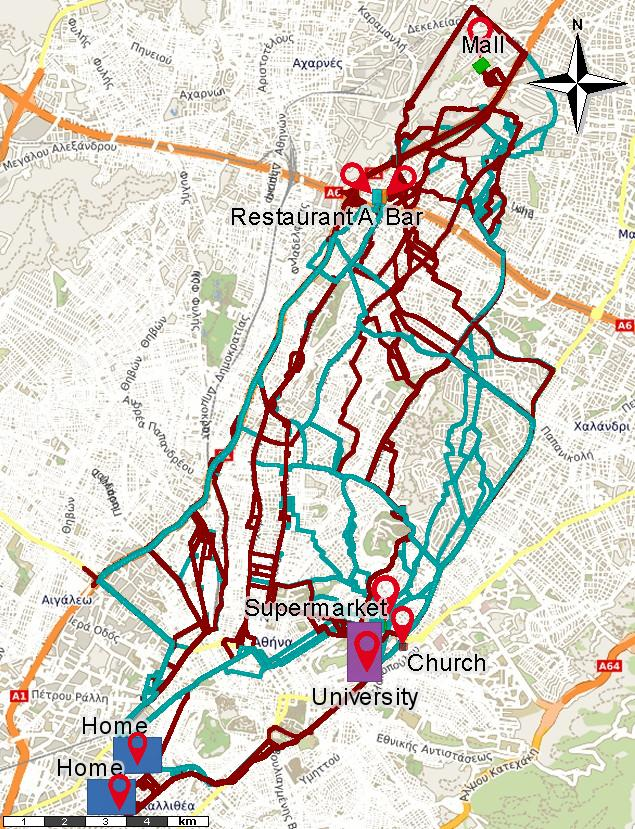
\includegraphics[width=.4\textwidth]{Images/Hermoupolis-RawPoints.jpg}
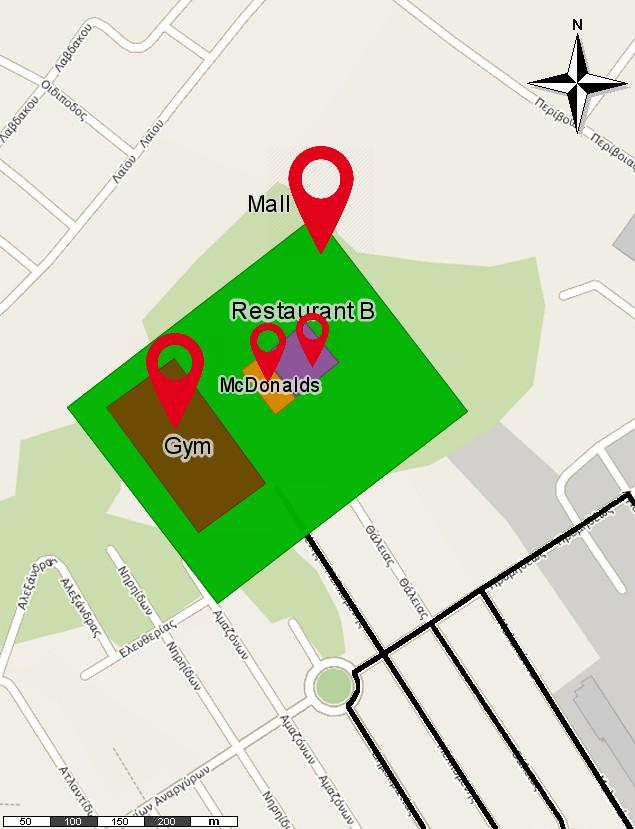
\includegraphics[width=.4\textwidth]{Images/Hermoupolis-CommercialCenter.jpg}
}
\caption{Hermoupolis generated trajectories (left). Mall area zoom in showing the stops inside mall. (right)}
\label{fig:hermoupolis_groundtruth}
\end{figure*}

\subsubsection{Results with the synthetic dataset}
Following the methodology used in previous experiments, we calculate the precision at recall for the 2 classes in the ground truth, comparing the results of SMSM with other measures. The dimensions used for the \emph{stops} are: a) spatial centroid of the \emph{stop}; b) temporal duration of the \emph{stop}; and c) the \emph{stop} name (Home, Mall, University, etc). For the \emph{moves} we used the activity performed by each moving object during the \emph{move} between two consecutive \emph{stops}.

%In this experiment we compared SMSM only with similarity measures developed for semantic trajectories, since the dimensions used are semantically enriched information of the \emph{stop} or the \emph{move} itself, unlike the two previous experiments where the \emph{move} was compared through the raw points of the \emph{move}.

For measuring the \emph{stops} similarity, we use: (i) the Euclidean distance for space; (ii) the proportion of the intersection between the time intervals of two \emph{stops}, as given by Equation \ref{func:time_interval}; and (iii) 1 and 0 for the semantics in case of exact match or no match, respectively. For the \emph{moves}, we consider the activity performed by the moving object during the \emph{move}, where 1 in the case of exact match and 0 otherwise. The weights for the \emph{stops} and the \emph{moves} are the same ($1/2$), and the weights of the \emph{stops} dimensions are $1/3$ for space, time, and semantics.

Table \ref{tab:hermoupolis_thresholds} presents the thresholds used for each measure. As the previous experiments, we define the thresholds for each dimension after we have experienced a range of values in each dimension (space and time), and the best results are reported for each measure.

\begin{table}[!h]
\scriptsize
  \centering
  \begin{tabular}{|c|c|c|c|}
  	\hline
  & \multicolumn{2}{c|}{Semantic trajectories} & \multicolumn{1}{c|}{Raw trajectories} \\
 	\cline{2-4}
  & Space (meters)& Time (intersection proportion) & Space (meters) \\
  	\hline
 SMSM & 300 & 0.1 & - \\
 MSM & 300 & 0.2 & - \\
 LCSS & 100 & 0.2 & 8 \\
 EDR & 100 & 0.2 & 8 \\
    \hline
  \end{tabular}
  \caption{Thresholds used for each measure}
  \label{tab:hermoupolis_thresholds}
\end{table}

Table \ref{tab:hermoupolis_measures_map_auc} presents the experimental results. SMSM outperforms all other measures. Comparing with measures for semantic trajectories, SMSM being around 12\% more precise than LCSS (0.82), EDR (0.82) and MSM (0.81). The other measures for semantic trajectories had worse results, with MAP scores of 0.40 and 0.33 for MSTP and CVTI, respectively. 


\begin{table}[h]
\scriptsize
  \centering
  \begin{tabular}{|l|c|c|c|c|}
  	\hline
 & \multicolumn{2}{c}{Semantic} & \multicolumn{2}{|c|}{Raw} \\
 	\cline{2-5}
 & MAP & AUC & MAP & AUC \\
  	\hline
SMSM & \textbf{0.93} & \textbf{0.94} & - & -\\
EDR & 0.82 & 0.85 & 0.51 & 0.54 \\
LCSS & 0.82 & 0.85 & 0.44 & 0.47 \\
MSM & 0.81 & 0.83 & - & - \\
MSTP & 0.40 & 0.44 & - & - \\
DTWa & - & - & 0.45 & 0.48 \\
CVTI & 0.33 & 0.37 & - & - \\
wDF & - & - & 0.35 & 0.39 \\
UMS & - & - & 0.29 & 0.33 \\
    \hline
  \end{tabular}
  \caption{MAP and AUC evaluation for the Hermoupolis dataset}
  \label{tab:hermoupolis_measures_map_auc}
\end{table}

Figure \ref{fig:hermoupolis_precision_recall} (left) shows the precision at recall curves for similarity measures for semantic trajectories, and SMSM is more accurate at each level. EDR, LCSS, and MSM had similar results because they do not take into account the \emph{moves}, not being able to distinguish the moves between the \emph{stops}, because the semantics of the moves distinguish the trajectories, and only the \emph{stops} are not sufficient. Despite this, these measures have a good MAP score mainly because the profiles are highly discriminative, where a behavior of a profile is basically exclusive of that profile, sharing few places in the same space and time with other profiles. All the remaining measures present worse results, since they do not take into account other dimensions when comparing the semantic trajectories.

\begin{figure*}[ht!]
\centerline{
\centering
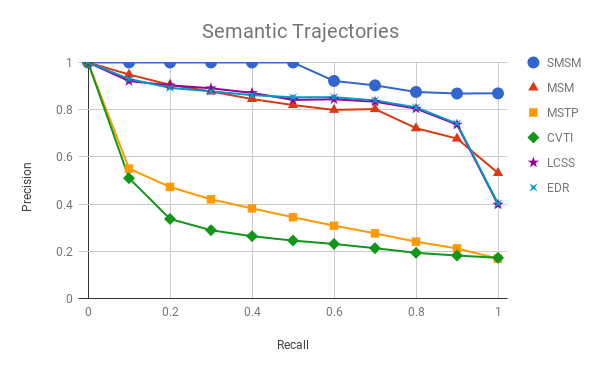
\includegraphics[width=.45\textwidth]{Images/P_R-chart_Hermoupolis_semantic.png}
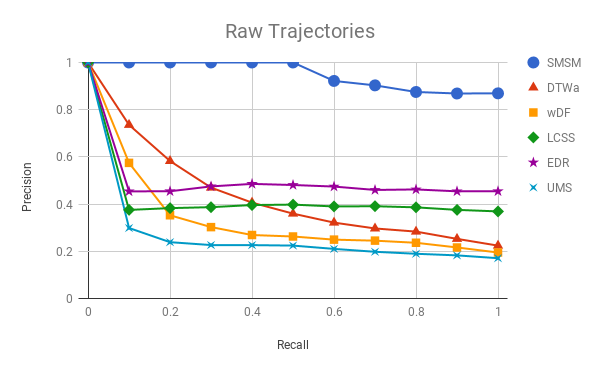
\includegraphics[width=.45\textwidth]{Images/P_R-chart_Hermoupolis_raw.png}
}
\caption{Precision at recall results for Hermoupolis semantic (left) and raw (right) trajectories}
\label{fig:hermoupolis_precision_recall}
\end{figure*}

Figure \ref{fig:hermoupolis_precision_recall} (right) shows the precision at recall curves for similarity measures for raw trajectories, and SMSM is still more accurate that all measures. In this dataset, all similarity measures for raw trajectories had poor results. It happens because the generated trajectories of distinct classes are spatially near, with the semantic being more relevant to discriminate the classes than the spatial dimension.

\subsection{Parameter Analysis}\label{sec:sensitivity}
 % in one or more dimensions. In case of (i), as SMSM is the first similarity measure to taking in account both \emph{stops} and \emph{moves}, we consider important for user to define the importance degree of the \emph{moves} in the application. In the case of (ii), the previous MSM similarity measure defines the importance degree of the dimensions by a sensibility analysis made by user, defining how much important is a dimension than other dimensions in the application. In the case of (iii), SMSM, as all other threshold-based similarity measures (LCSS, EDR, MSM, etc), needs the \emph{threshold} values to define if two points match in one or more dimensions. These values are application dependant and must be fine-tuned by user. Besides that, a robust similarity measure should be resilient through those values.
%The decision of correct weights needs a sensitivity analysis about the problem analyzed and the used data.
\hl{SMSM has two important groups of parameters: i) the \emph{weights} to define the importance of stops/moves and dimensions; and ii) the \emph{thresholds} to define if two points match.
With the weights framework, SMSM is flexible to give more or less importance to the stops, moves, and dimensions. %In applications where space is more important, this dimension may have a higher weight. This is the case for applications where the location or the position of the objects matter (e.g. wildlife monitoring, traffic conditions, road network analysis, car sharing, etc). In applications where the location is less important but the semantics of the places is more relevant as the flow of objects that visit specific types of places (e.g. touristic places, japonese restaurants, etc) then the semantic dimension needs a higher weight.

To show the impact of the weight parameters on the similarity analysis, we evaluate the \emph{weight} of the \emph{stops} and the \emph{moves} in all experimental datasets. Table {\ref{tab:sensibility_stopmove}} shows the results for the weight varying from 0 to 1, where 0 means that the moves will be ignored and 1 means that only the moves will be considered.  As can be seen, if the influence of the \emph{moves} is ignored, i.e., weight = 0, SMSM reaches a MAP score of only $0.74$ in the Geolife dataset, $0.49$ in the Taxi dataset, and $0.75$ in the synthetic dataset, indicating a confusion between the similarity of the trajectories that are discriminated by the moves. The best result is achieved when the weight of the \emph{moves} is greather than zero and less or equal than 1, achieving a MAP score of $0.95$ in the Geolife, $0.71$ in the Taxi dataset, and $0.96$ in the synthetic dataset, indicating that the \emph{moves} should be considered in these datasets.}

\begin{table}[ht!]
  \scriptsize
  \centering
  \begin{tabular}{|c|c|c|c|c|}
  	\hline
Stop weight & Move weight & Geolife (MAP) & Taxi (MAP) & Hermoupolis (MAP) \\
  	\hline
0.00 & 1.00 & \textbf{0.95} & 0.66 & \textbf{0.96}\\
0.25 & 0.75 & \textbf{0.95} & 0.66 & 0.93\\
0.50 & 0.50 & \textbf{0.95} & 0.70 & 0.93\\
0.75 & 0.25 & \textbf{0.95} & \textbf{0.71} & 0.89\\
1.00 & 0.00 & 0.74 & 0.49 & 0.75 \\
    \hline
  \end{tabular}
  \caption{Impact of the weights over the moves in trajectory similarity}
  \label{tab:sensibility_stopmove}
\end{table}

\hl{Table {\ref{tab:sensibility_spatial_thresholds}} shows the similarity score of SMSM when the spatial threshold for the stops varies from 50 to 2,000 meters on both datasets. As can be observed, there is not much variation in the results, but this is because the stops are more or less the same in all trajectories. The exception is the synthetic dataset, where a larger spatial threshold ($2,000$ meters) does the retrieval results to reach a lower MAP score ($0.83$). This is because in this dataset there are many more stops than other datasets, with many of them close to other stops.}

\begin{table}[ht!]
  \scriptsize
  \centering
  \begin{tabular}{|l|c|c|c|}
  	\hline
Threshold (meters) & Geolife (MAP) & Taxi (MAP) & Hermoupolis (MAP)\\
  	\hline
50 & \textbf{0.95} & \textbf{0.70} & 0.90\\
100 & 0.95 & \textbf{0.70}  & 0.90\\
300 & 0.95 & \textbf{0.70} & \textbf{0.93} \\
500 & 0.94 & \textbf{0.70} & \textbf{0.93}\\
1000 & 0.94 & \textbf{0.70} & 0.90\\
2000 & 0.94 & \textbf{0.70} & 0.83\\
    \hline
  \end{tabular}
  \caption{The MAP score for the spatial threshold variation from 50 up to 2,000 meters}
  \label{tab:sensibility_spatial_thresholds}
\end{table}

\hl{It is worth mentioning that almost all similarity measures for either raw or semantic trajectories need the definition of thresholds to define how far or how close are two trajectory elements. This is not an exclusive need of SMSM. }

\section{Discussion: Applications versus Measures}\label{sec:discussion}


\hl{Trajectory data can have several formats. Depending on the format and the application requirements, different trajectory analysis and mining methods will be needed, and so different similarity measures can be applied. For applications that use raw GPS data, as trajectories of taxis, buses, or cars, with the intend to detect, for instance, traffic conditions or traffic jams, the most appropriate measure is UMS. UMS outperformed all measures for raw trajectories, because it is robust to trajectories with different sampling rates or different distances between trajectory points (the case when a trajectory varies the speed in a city), because instead of using a radius around each trajectory point to find the similar trajectories in the spatial neighbourhood, it uses ellipses between every two trajectory points, and the size of the ellipses is dinamically defined based on the distance between two trajectory points. UMS is not so good in high sampled trajectories, where the ellipsis are very small, and in this case DTWa is  a good choice and outperformed UMS in the pedestrian trajectories of Geolife used in our experiments.}

\hl{For applications that use GPS trajectories annotated only with stops or where the moves are not important, or trajectories extracted from social media data, which are more sparse and that do not have moves, the best measure is MSM. MSM is useful in applications where one is interested in finding users that visit the same places, at similar times, but where the order of the visits is not important. In tourism applications where the analyst wants to find similar tourist trajectories to either predict or to recommend the next place to be visited, MSM is not appropriate because it ignores the order. When the sequence of the visited places is important, even when the details about the moves are not, SMSM is more appropriate, because it considers the order of the stops.}

\hl{For dealing with GPS trajectories enriched with both stops and moves, and the spatial, temporal or semantic characteristcs of both stops and moves are important, SMSM is the most appropriate measure. In a tourism application, for instance, where the tourist has a time constraint to visit a city, a sequence of visits can be recommended based on the similarity analysis of other tourists that visited the same city. SMSM is also the most appropriate measure in applications that need the most similar paths or popular routes between stops.}
%but considering the visited places and the moves between the stops, in order to estimate the duration of the different movements between the stops. SMSM is the best measure for traffic analysis where the objective is to compare the traffic along  different paths that connect two regions in a city.}

\hl{It is important to emphasize that in applications where the spatial movement of the moves is important, i.e., the raw trajectory points, SMSM can use the UMS for the move similarity when trajectories have low sampling rate and DTW when trajectories have high sampling rate.}

%This study was financed in part by the Coordenação de Aperfeiçoamento de Pessoal de Nível Superior - Brasil (CAPES) - Finance Code 001

\section{Conclusion} \label{sec:conclusions}
In this work we proposed SMSM, a new similarity measure for semantic trajectories that supports both stops and moves.  To the best of our knowledge, SMSM is the first semantic trajectory similarity measure that deals with both stops and moves and their space, time and semantic dimensions. The proposed similarity measure is robust  to consider multiple dimensions of stops and moves, where a move, for instance, can be represented as raw points, the traveled distance, the major direction, the names of streets, the transportation mode, etc.

SMSM supports the definition of weights for stops, moves and dimensions, so the measure is flexible to give more or less importance for specific parts of trajectories. On the other hand, these weights may be difficult to estimate from the user point of view, but in case he has no knowledge about the domain, the best is to define the same weight for all elements.

We performed experiments using real \hl{and synthetic} data of distinct contexts, including car trajectories and pedestrian trajectories. By evaluating SMSM with an information retrieval approach, we show that SMSM was more accurate than other measures developed either for raw or semantic trajectories.

SMSM requires a full spatial match between the start and end stop of two movement elements to evaluate the move. In future works we will study an extension of SMSM to evaluate the move in cases where the end stops of two movement elements do not have a match.

\bibliographystyle{tfv}
\bibliography{sbc-template}

\end{document}